% Sablon pentru realizarea lucrarii de licenta, conform cu recomandarile
% din ghidul de redactare:
% - https://fmi.unibuc.ro/finalizare-studii/
% - https://drive.google.com/file/d/1xj9kZZgTkcKMJkMLRuoYRgLQ1O8CX0mv/view

% Multumiri lui Gabriel Majeri, acest sablon a fost creat pe baza
% codului sursa a lucrarii sale de licenta. 
% Codul sursa: https://github.com/GabrielMajeri/bachelors-thesis
% Website: https://www.gabrielmajeri.ro/
%
% Aceast sablon este licentiat sub Creative Commons Attribution 4.0 International License.

\documentclass[12pt, a4paper]{report}

% Suport pentru diacritice și alte simboluri
\usepackage{fontspec}
\usepackage{underscore}

% Suport pentru mai multe limbi
\usepackage{polyglossia}

% Setează limba textului la română
\setdefaultlanguage{romanian}
% Am nevoie de engleză pentru rezumat
\setotherlanguages{english}

% Indentează și primul paragraf al fiecărei noi secțiuni
\SetLanguageKeys{romanian}{indentfirst=true}

% Suport pentru diferite stiluri de ghilimele
\usepackage{csquotes}

\DeclareQuoteStyle{romanian}
  {\quotedblbase}
  {\textquotedblright}
  {\guillemotleft}
  {\guillemotright}

% Utilizează biblatex pentru referințe bibliografice
\usepackage[
    maxbibnames=50,
    sorting=nty
]{biblatex}

\addbibresource{bibliography.bib}

% Setează spațiere inter-linie la 1.5
\usepackage{setspace}
\onehalfspacing

% Modificarea geometriei paginii
\usepackage{geometry}

% Include funcțiile de grafică
\usepackage{graphicx}
\usepackage{tabularx}
\usepackage{multirow}
% Încarcă imaginile din directorul `images`
\graphicspath{{./images/}}

% Listări de cod
\usepackage{listings}
\usepackage{color}
\usepackage{svg}

\definecolor{dkgreen}{rgb}{0,0.6,0}
\definecolor{gray}{rgb}{0.5,0.5,0.5}
\definecolor{mauve}{rgb}{0.58,0,0.82}

\lstdefinestyle{yaml}{
  aboveskip=3mm,
  belowskip=3mm,
  showstringspaces=false,
  columns=flexible,
  basicstyle={\small\ttfamily},
  numberstyle=\tiny\color{gray},
  keywordstyle=\color{blue},
  commentstyle=\color{dkgreen},
  stringstyle=\color{mauve},
  breaklines=true,
  breakatwhitespace=true,
  tabsize=2
}

\lstdefinestyle{java}{frame=tb,
  language=Java,
  aboveskip=3mm,
  belowskip=3mm,
  showstringspaces=false,
  columns=flexible,
  basicstyle={\small\ttfamily},
  numberstyle=\tiny\color{gray},
  keywordstyle=\color{blue},
  commentstyle=\color{dkgreen},
  stringstyle=\color{mauve},
  breaklines=true,
  breakatwhitespace=true,
  tabsize=2
}

% Linkuri interactive în PDF
\usepackage[
    colorlinks,
    linkcolor={black},
    menucolor={black},
    citecolor={black},
    urlcolor={blue}
]{hyperref}

% Simboluri matematice codificate Unicode
\usepackage[warnings-off={mathtools-colon,mathtools-overbracket}]{unicode-math}

% Comenzi matematice
\usepackage{amsmath}
\usepackage{mathtools}

%figures
\usepackage{float}

% Formule matematice
\newcommand{\bigO}[1]{\symcal{O}\left(#1\right)}
\DeclarePairedDelimiter\abs{\lvert}{\rvert}

% Suport pentru rezumat în două limbi
% Bazat pe https://tex.stackexchange.com/a/70818
\newenvironment{abstractpage}
  {\cleardoublepage\vspace*{\fill}\thispagestyle{empty}}
  {\vfill\cleardoublepage}
\renewenvironment{abstract}[1]
  {\bigskip\selectlanguage{#1}%
   \begin{center}\bfseries\abstractname\end{center}}
  {\par\bigskip}

% Suport pentru anexe
\usepackage{appendix}

% Stiluri diferite de headere și footere
\usepackage{fancyhdr}

% Metadate
\title{Aplicație web pentru gestionarea eficientă a angajaților și a sarcinilor de lucru}
\author{Alexandra-Diana Ciocan}

% Generează variabilele cu @
\makeatletter

\begin{document}

% Front matter
\cleardoublepage
\let\ps@plain

% Pagina de titlu
\begin{titlepage}

% Redu marginile
\newgeometry{left=2cm,right=2cm,bottom=1cm}

\begin{figure}[!htb]
    \centering
    \begin{minipage}{0.2\textwidth}
        
\includegraphics[width=\linewidth]{logo-ub.png}
    \end{minipage}
    \begin{minipage}{0.5\textwidth}
        \large
        \vspace{0.2cm}
        \begin{center}
            \textbf{UNIVERSITATEA DIN BUCUREȘTI}
        \end{center}
        \vspace{0.3cm}
        \begin{center}
            \textbf{
                FACULTATEA DE \\
                MATEMATICĂ ȘI INFORMATICĂ
            }
        \end{center}
    \end{minipage}
    \begin{minipage}{0.2\textwidth}
        
\includegraphics[width=\linewidth]{logo-fmi.png}
    \end{minipage}
\end{figure}

\begin{center}
\textbf{SPECIALIZAREA INFORMATICĂ}
\end{center}

\vspace{1cm}

\begin{center}
\Large \textbf{Lucrare de licență}
\end{center}

\begin{center}
\huge \textbf{\MakeUppercase{\@title}}
\end{center}

\vspace{3cm}

\begin{center}
\large \textbf{Absolvent \\ \@author}
\end{center}

\vspace{0.25cm}

\begin{center}
\large \textbf{Coordonator științific \\ Lect.dr. Natalia Gabriela Ozunu}
\end{center}

\vspace{2cm}

\begin{center}
\Large \textbf{București, iunie 2024}
\end{center}
\end{titlepage}
\restoregeometry
\newgeometry{
    margin=2.5cm
}

\fancypagestyle{main}{
  \fancyhf{}
  \renewcommand\headrulewidth{0pt}
  \fancyhead[C]{}
  \fancyfoot[C]{\thepage}
}

\addtocounter{page}{1}

% Rezumatul
\begin{abstractpage}

\begin{abstract}{romanian}
Lorem ipsum dolor sit amet, consectetur adipiscing elit. Fusce vitae eros sit amet sem ornare varius. Duis eget felis eget risus posuere luctus. Integer odio metus, eleifend at nunc vitae, rutrum fermentum leo. Quisque rutrum vitae risus nec porta. Nunc eu orci euismod, ornare risus at, accumsan augue. Ut tincidunt pharetra convallis. Maecenas ut pretium ex. Morbi tellus dui, viverra quis augue at, tincidunt hendrerit orci. Lorem ipsum dolor sit amet, consectetur adipiscing elit. Aliquam quis sollicitudin nunc. Sed sollicitudin purus dapibus mi fringilla, nec tincidunt nunc eleifend. Nam ut molestie erat. Integer eros dolor, viverra quis massa at, auctor.
\end{abstract}

\begin{abstract}{english}
Lorem ipsum dolor sit amet, consectetur adipiscing elit. Fusce vitae eros sit amet sem ornare varius. Duis eget felis eget risus posuere luctus. Integer odio metus, eleifend at nunc vitae, rutrum fermentum leo. Quisque rutrum vitae risus nec porta. Nunc eu orci euismod, ornare risus at, accumsan augue. Ut tincidunt pharetra convallis. Maecenas ut pretium ex. Morbi tellus dui, viverra quis augue at, tincidunt hendrerit orci. Lorem ipsum dolor sit amet, consectetur adipiscing elit. Aliquam quis sollicitudin nunc. Sed sollicitudin purus dapibus mi fringilla, nec tincidunt nunc eleifend. Nam ut molestie erat. Integer eros dolor, viverra quis massa at, auctor.
\end{abstract}

\end{abstractpage}

\tableofcontents

% Main matter
\cleardoublepage
\pagestyle{main}
\let\ps@plain\ps@main

\chapter{Introducere}

\section{Lorem ipsum}

Lorem ipsum dolor sit amet \cite{fake_citation}, consectetur adipiscing elit. Nam convallis dapibus ante in interdum. Aliquam vitae elit eu elit gravida facilisis. Proin tincidunt sodales elit vitae ornare. Suspendisse quis rutrum ipsum, eget tempor felis. Nulla facilisi. Vivamus mollis quam a est aliquam congue. Nulla risus turpis, rutrum ac lacus molestie, vestibulum ultricies enim. Suspendisse a urna ultrices quam pulvinar finibus ac vitae felis. Ut sit amet interdum lacus. Sed in cursus arcu. Vivamus quis eros efficitur, ullamcorper dui ut, blandit nisl. Interdum et malesuada fames ac ante ipsum primis in faucibus. Nunc interdum venenatis mi, sed placerat elit feugiat in. Praesent dignissim ante nec rutrum tempus.

Aenean accumsan nunc nunc, nec maximus ex ultricies et. In porta sollicitudin augue. Curabitur consectetur elit nec eros laoreet fermentum. Vivamus nec nisl a lectus scelerisque viverra at id tortor. Fusce et erat dictum, dictum odio nec, aliquam orci. Vestibulum gravida feugiat purus. Mauris non neque est. Sed commodo vel enim vel tincidunt. Sed faucibus dolor id dui dictum pellentesque. Vestibulum ante ipsum primis in faucibus orci luctus et ultrices posuere cubilia curae; Mauris interdum tempor purus ut tempor. Maecenas ac suscipit ex. Sed vitae diam nec neque ultricies faucibus. In at purus elit. Nunc placerat nunc tortor.

Fusce fermentum quis tellus vitae congue. Interdum et malesuada fames ac ante ipsum primis in faucibus. Proin convallis congue sapien semper volutpat. Curabitur rhoncus et nunc quis tempor. Quisque sollicitudin dolor id varius luctus. Donec sapien dolor, eleifend quis justo id, euismod ultrices nulla. Suspendisse leo quam, luctus in velit ac, venenatis molestie odio. Aliquam vitae feugiat elit. Sed auctor gravida leo, ut dictum enim tempus non. Suspendisse in dapibus urna, vitae pretium ligula. Morbi ut diam laoreet, convallis leo non, semper arcu. Sed vel lorem tortor. In auctor a diam sit amet convallis. Etiam ipsum ligula, luctus quis interdum ac, consequat vitae orci. Maecenas hendrerit turpis tristique, tincidunt nisi ut, mattis augue.

\section{Dolor sit amet}

Fusce fermentum quis tellus vitae congue. Interdum et malesuada fames ac ante ipsum primis in faucibus. Proin convallis congue sapien semper volutpat. Curabitur rhoncus et nunc quis tempor. Quisque sollicitudin dolor id varius luctus. Donec sapien dolor, eleifend quis justo id, euismod ultrices nulla. Suspendisse leo quam, luctus in velit ac, venenatis molestie odio. Aliquam vitae feugiat elit. Sed auctor gravida leo, ut dictum enim tempus non. Suspendisse in dapibus urna, vitae pretium ligula. Morbi ut diam laoreet, convallis leo non, semper arcu. Sed vel lorem tortor. In auctor a diam sit amet convallis. Etiam ipsum ligula, luctus quis interdum ac, consequat vitae orci. Maecenas hendrerit turpis tristique, tincidunt nisi ut, mattis augue.

\subsection{Quis tellus vitae}

Aenean accumsan nunc nunc, nec maximus ex ultricies et. In porta sollicitudin augue. Curabitur consectetur elit nec eros laoreet fermentum. Vivamus nec nisl a lectus scelerisque viverra at id tortor. Fusce et erat dictum, dictum odio nec, aliquam orci. Vestibulum gravida feugiat purus. Mauris non neque est. Sed commodo vel enim vel tincidunt. Sed faucibus dolor id dui dictum pellentesque. Vestibulum ante ipsum primis in faucibus orci luctus et ultrices posuere cubilia curae; Mauris interdum tempor purus ut tempor. Maecenas ac suscipit ex. Sed vitae diam nec neque ultricies faucibus. In at purus elit. Nunc placerat nunc tortor.
\chapter{Preliminarii}

\section{Funcționalități principale}
\subsection{Actori}
Principalii actori ai cazurilor de utilizare sunt: 

- Membru de echipă

- Manager

- Administrator

\subsection{Cazuri uzuale de utilizare}
\begin{itemize}
\item Manager:

1. În calitate de manager, aș vrea să adaug sarcini de lucru pentru echipa mea, cu detalii despre criteriile de acceptanță, prioritate, dificultate și termen limită, pentru ca acestea să fie cât mai clare pentru membri echipei.

2. În calitate de manager, aș vrea să pot vizualiza factorii de performanță precum disponibilitatea, volumul de muncă, calificarea, eficiența și atribuțiile fiecărui membru al echipei mele, pentru a evalua corect atribuirea de sarcini de lucru noi.

3. În calitate de manager, aș vrea să pot modifica factorii de performanță precum disponibilitatea, volumul de muncă, calificarea, eficiența și atribuțiile fiecărui membru al echipei mele, pentru ca aceștia să fie mereu actuali.

4. În calitate de manager, aș vrea să atribui automat sarcini de lucru, bazat pe detaliile sarcinii de lucru și pe factorii de performanță angajatului, pentru a le împărți cât mai echitabil și a maximiza productivitatea și șansele ca sarcina să fie îndeplinită până la
termen.

5. În calitate de manager, aș vrea să pot atribui manual sarcini de lucru, bazat pe analiza mea asupra situației, pentru a ajusta eventualele erori ale recomandărilor, a adapta panoul la noi informații relative la disponibilitate, sau a încuraja creșterea/scăderea productivității pentru un anumit membru al echipei

\item Employee:

1. În calitate de angajat obișnuit, aș vrea să îmi vizualizez sarcinile de lucru împreuna cu detalii despre criteriile de acceptanță, prioritate, dificultate și termen limită, pentru a îmi putea organiza activitatea zilnică.

2. În calitate de angajat obișnuit, aș vrea să pot actualiza statusul sarcinilor de lucru pentru ca managerul meu să le cunoască progresul.

3. În calitate de angajat obișnuit, aș vrea să fiu notificat atunci când managerul îmi atribuie o sarcina de lucru nouă, pentru a percepe mai ușor schimbări ale panoului cu sarcinile mele.

\item Administrator:

1. În calitate de administrator, aș vrea să pot crea, actualiza sau elimina utilizatori și echipe, pentru a putea gestiona accesul la platformă și organizarea internă.

2. În calitate de administrator, aș vrea să pot atribui manageri echipelor create, pentru ca fiecare echipă să fie gestionată de un manager.

\end{itemize}


\section{Alegerea tehnologiilor}

\subsection{Typescript\&React}

Pentru partea de front-end a aplicației web am ales să utilizez Typescript ca limbaj și React ca bibliotecă, împreună cu componente reutilizabile din biliboteca de componente UI Ant Design.

Utilizarea limbajului Typescript, în defavoarea limbajului JavaScript, este explicată prin minimizarea erorilor cauzate de inconsistența adusă de faptul ca JavaScript este un limbaj „loosely typed” („dinamically typed”) și de incertitudinea adusă de acest fapt. Astfel, prezența interfețelor și tipurilor de date bine stabilite facilitează dezvoltarea rapidă și stabilă.

În plus, biblioteca React aduce o perspectivă structurată dezvoltării interfeței, prin definirea de componente reutilizabile în cadrul aplicației. O parte din componentele UI sunt utilizate din biblioteca Ant Design, folositoare prin aspectul vizual unitar și formal, acompaniat de o documentație bine pusă la punct. Un dezavantaj al abordării prin componente este comunicarea între acestea, motiv pentru care am folosit state managerul MobX. 

\subsection{Java\&Spring}

Pentru partea de back-end a aplicației web am optat pentru limbajul Java și framework-ul Spring și ecosistemul acestuia, având în vedere opțiunile robuste pentru gestionarea logicii de afaceri, a securității și a interacțiunilor cu baza de date.

Versiunea de Java utilizată este Java 21, pentru a avea acces la cele mai noi update-uri ale limbajului, cu cele mai noi feature-uri, precum clase Record, fire virtuale de execuție, și Sequenced Collections. 

Versiunea de Spring folosită este 6.1.3, ce vine împreună cu Spring Boot 3.2.2, alături de alte dependințe, printre cele mai notabile numărându-se Spring Security și Jakarta Persistence API (JPA).

Cele mai majore utilități puse la dispoziție de Spring și de ecosistemul de dependințe sunt:

- securitatea asigurată prin generarea de JSON Web Tokens pentru autentificarea și autorizarea utilizatorilor și a cererilor HTTP trimise;

- crearea tabelelor și conectarea la baza de date facilitată de ORM-ul JPA;

- injectarea dependințelor prin constructorii claselor, în scopul reducerii codului boilerplate.

[detaliere spring boot, spring security, spring jpa]

\subsection{PostgreSQL}

Pentru persistența datelor am ales PostgreSQL, un sistem open-source de gestiune pentru baze de date, pentru sistemul său robust de asigurare a integrității datelor și abilitatea de a manevra ușor cantități mari de date.
\chapter{Arhitectura aplicației}

\section{Microservicii}

Aplicația adoptă paradigma arhitecturală a microserviciilor. Microserviciile presupun segmentarea unei aplicații într-o suită de servicii specializate, independente, ce comunică prin protocoale light-weight. Pentru comunicare am ales cea mai populară formă, API-urile bazate pe HTTP. Unul din avantajele principale ale acestei arhitecturi este decuplarea serviciilor implicate. Eșecul unui serviciu nu afectează întreaga aplicație, astfel încât problemele se manifestă izolat și sunt mai ușor de controlat. Un alt motiv pentru care am considerat că această arhitectură este potrivită aplicației este versatilitatea permisă în alegerea tehnologiilor și a limbajelor de programare\cite{building_microservices}.  Într-o aplicație monolit, această libertate nu ar fi fost posibilă.

 \begin{figure}[ht]
	\centering
 	 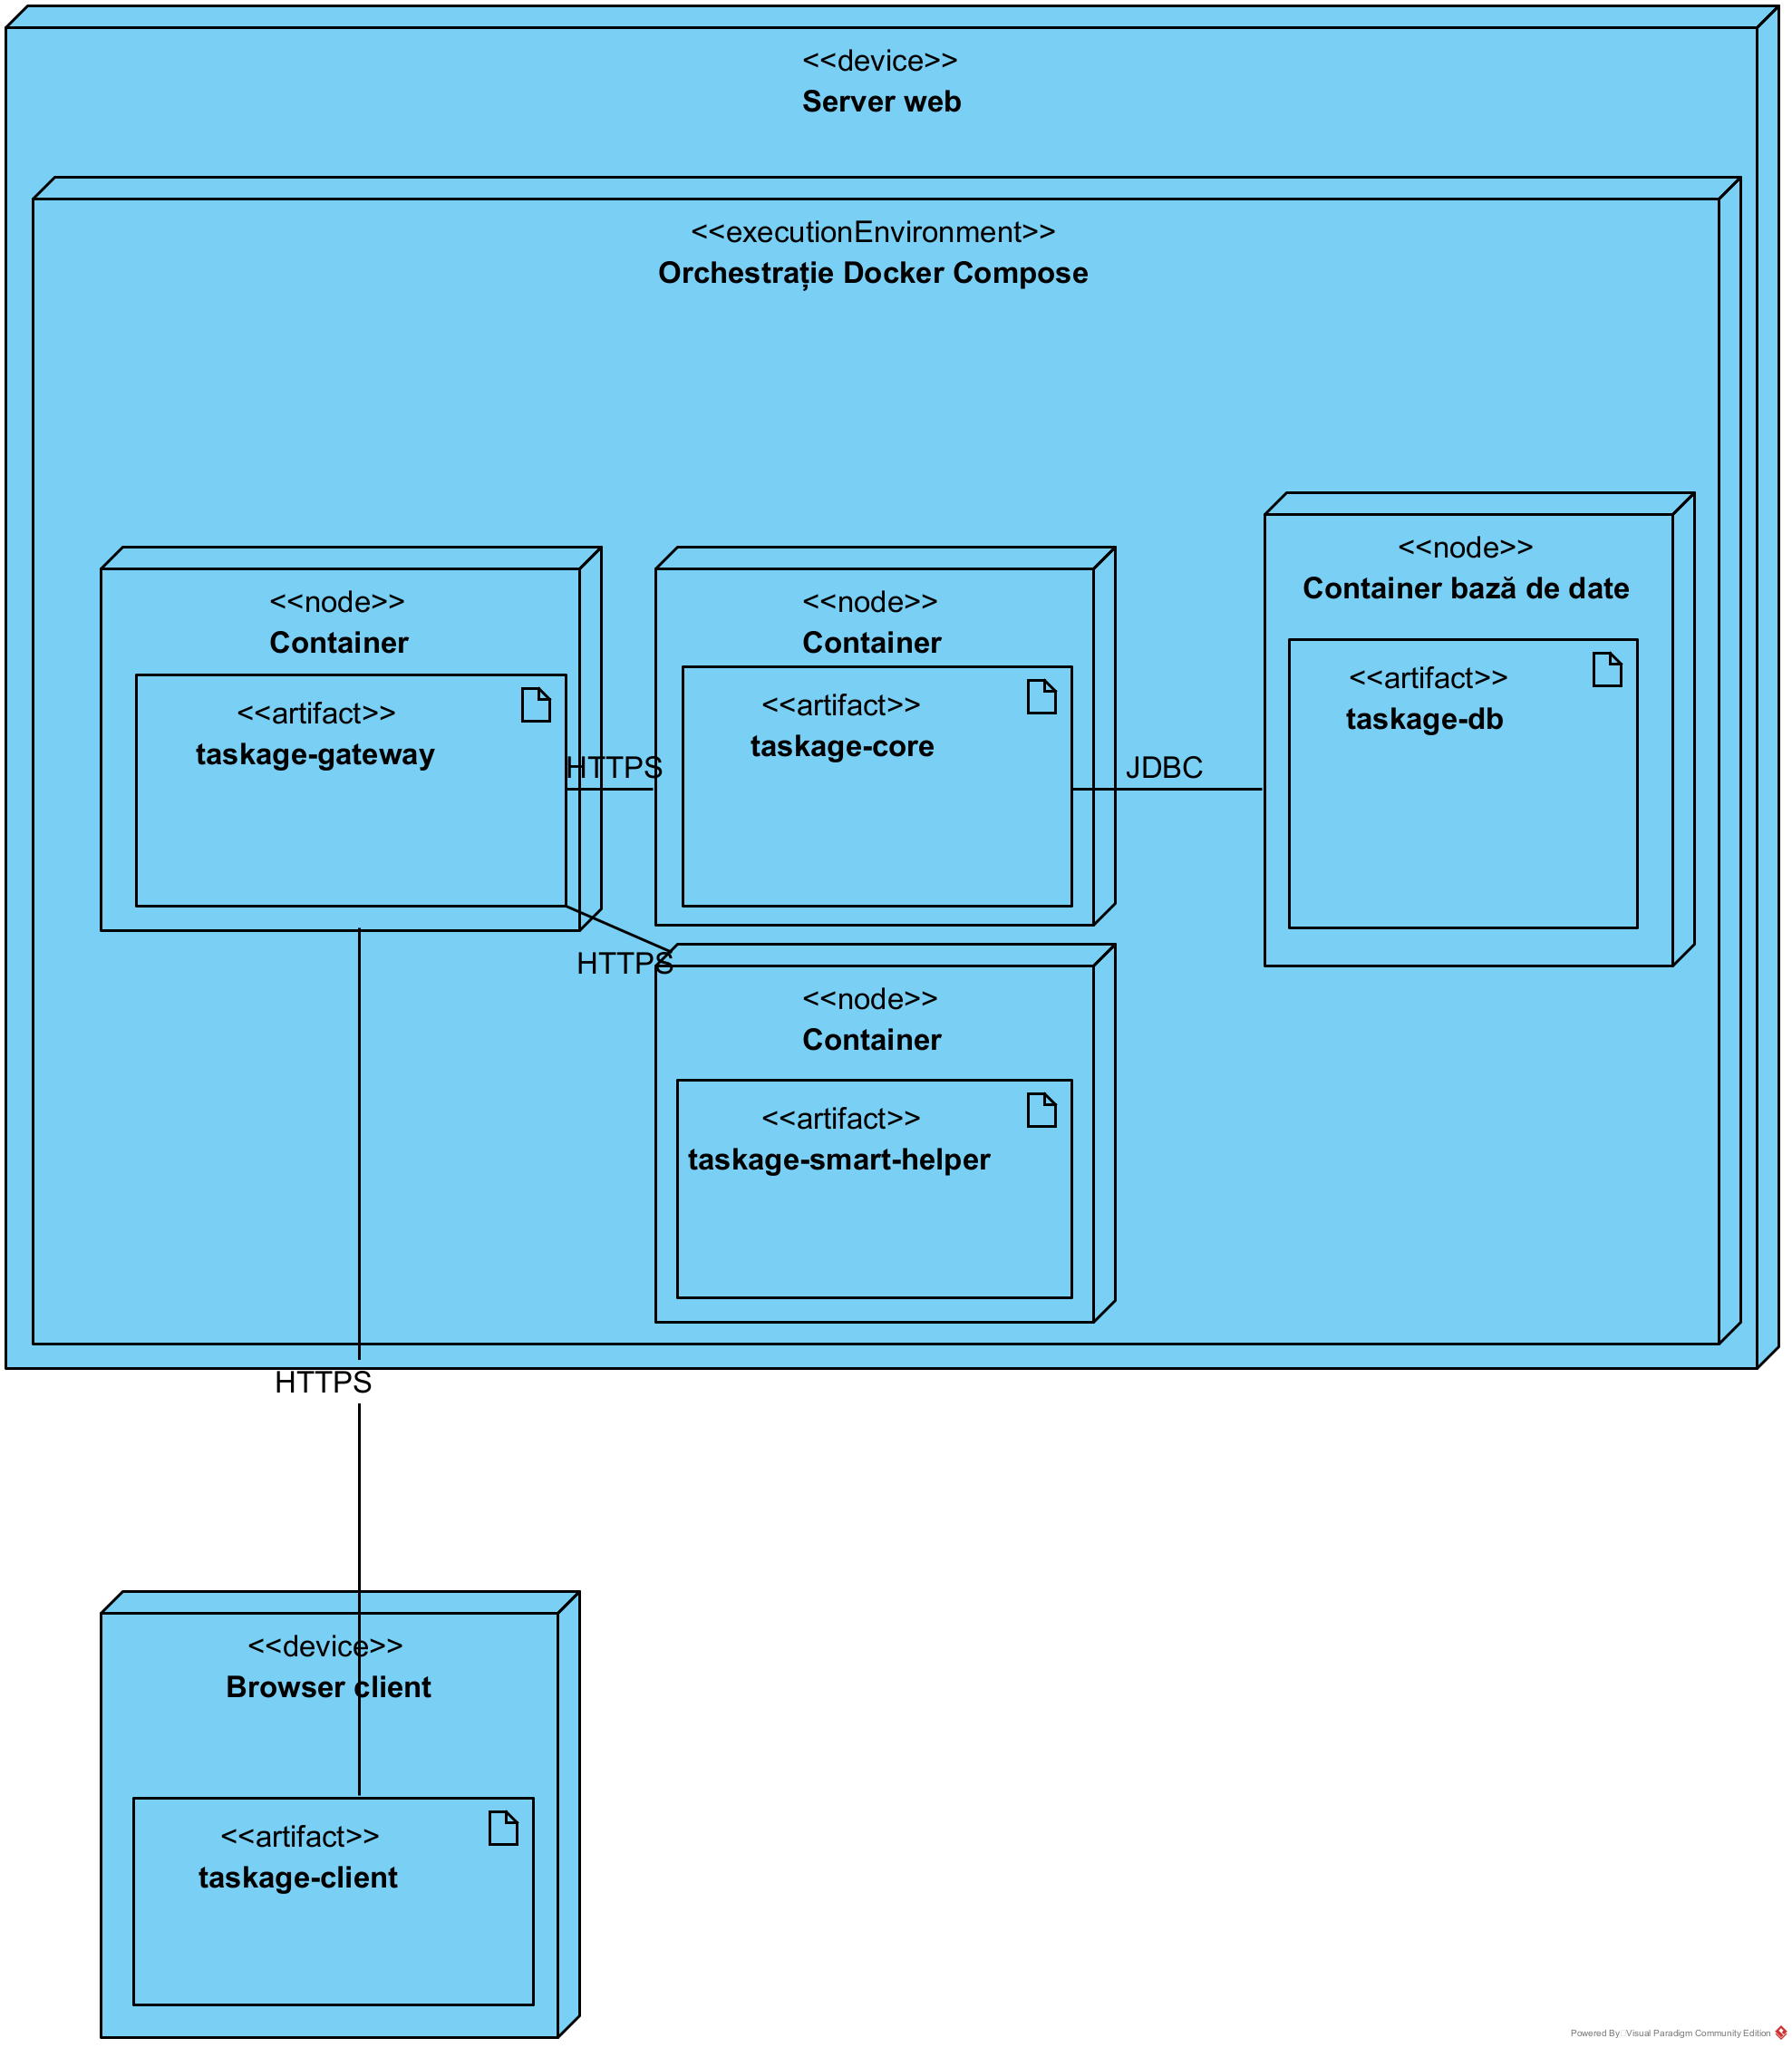
\includegraphics[width=\linewidth]{deployment-diagram.png}
	\caption{Diagrama de desfășurare}
	\label{fig:deployment-diagram}
 \end{figure}

Figura \ref{fig:deployment-diagram} ilustrează natura modulară a aplicației și integrarea diferitelor microservicii. Pe partea de front-end, artefactul aplicației React Taskage-Client rulează în browser-ul web al utilizatorului prin codul transpilat din TSX în JS. Acesta comunică cu serverul prin apeluri HTTP, utilizând componenta Spring Cloud Taskage-Gateway ca punct de intrare către functionalitățile back-end. Acest punct de intrare redirecționează apelurile spre componenta potrivită, pe baza configurărilor indicate în fișierul application.yml. Un gateway este un intermediar rafinat, oferind și posibilități de service discovery și load balancing. Apelul este trimis mai departe prin HTTP, iar conexiunile la baza de date sunt făcute prin JDBC pentru componenta Taskage-Core, respectiv toolkit-ul Flask-SQLAlchemy pentru componenta Taskage-Helper. Scopul componentei Taskage-Core este reprezentat de operațiile centrale aplicației, în principal CRUD, în timp ce componenta Taskage-Helper nu face decât operații de citire asupra bazei de date, scopul ei fiind analiza datelor stocate.

\section{Taskage-Gateway}

Un API gateway servește, în general, drept singurul punct de contact dintre aplicații externe sau interfețe utilizator și back-end-uri și este specific arhitecturii bazate pe microservicii. Aceasta gestionează cererile HTTP ce ajung la ea și le redirecționează, comportându-se ca un „om de mijloc” (middleman) între interfață și logica de afaceri sau sursa de date.  Cunoscut și sub denumirea de „reverse proxy”, poate analiza cererile primite și, în funcție de cale, headers și parametrii și poate decide încotro le va redirecționa.

Mai mult, API gateway-ul poate să gestioneze în mod eficient volumului de cereri ce ajunge către fiecare replică a unui serviciu, în cadrul unei arhitecturi bazată pe microservicii, pe baza unui algoritm de load balancing precum Round Robin, Least Connections, sau Weighted Distribution.

Există multe soluții pentru API gateway-uri ce necesită configurare minimă, ce vin de la toți giganții industriei Cloud (Google - Cloud Endpoints, Amazon - Amazon API Gateway, Microsoft - Azure API Gateway), însă există și soluții open-source, precum Apache APISIX API Gateway. În cadrul proiectului Taskage, este folosit Spring Cloud Gateway, fiind ușor de utilizat și configurat, necesitând în principal dependințe de Maven și un fișier de configurări, fișier de tip resursă, „application.yml”(figura \ref{fig:yaml}), în cadrul căruia sunt definite regulile de rutare aferente, sub secțiunea „cloud.gateway”.

Putem observa diverse componente de configurare: secțiunea routes prezintă configurările aferente rutării cererilor primite de către API gateway, sub care vine fiecare rută în parte, alături de URI-ul ei, și configurări adiționale, precum modelul căii cererii ce va intra pe această rută. În plus, se poate observa și secțiunea filters, sub care Spring Cloud Gateway îți permite să definești o gamă largă de filtre ce urmează să fie aplicate cererii, precum adăugarea de circuit breakere, rescrierea căii specifice sau prefixarea/sufixarea acesteia, sau, cum este cazul în configurarea prezentată, adăugarea unui header cu o valoare specifică pentru a valida că cererea a trecut întâi prin API Gateway și nu a fost făcută în mod direct endpoint-ului REST.

\begin{figure}[H]
	\begin{lstlisting}[frame=single, style=yaml]
  cloud:
    gateway:
      routes:
        - id: core
          uri: http://127.0.0.1:8080
          predicates:
            - Path=/**
          filters:
            - AddRequestHeader=X-XSRF-Token, ValidToken
      globalcors:
        cors-configurations:
          "[/**]":
            allowed-origins:
              - http://localhost:3000
            allowedMethods: "GET, POST, PUT, DELETE, OPTIONS"
            allowedHeaders: "Origin, X-Requested-With, Content-Type, Accept, Content-Length, TOKEN, Authorization"
            allowCredentials: true
            maxAge: 3600
	\end{lstlisting}
	\caption{application.yml}
	\label{fig:yaml}
\end{figure}

În plus, se pot face și configurări în ceea ce privește „cross-origin request forgery”, ce se pot configura per rută și vizează parametrii precum origini permise, metode HTTP permise și headere permise, ca măsură de securitate.

\section{Taskage-Core}

 \begin{figure}[ht]
	\centering
 	 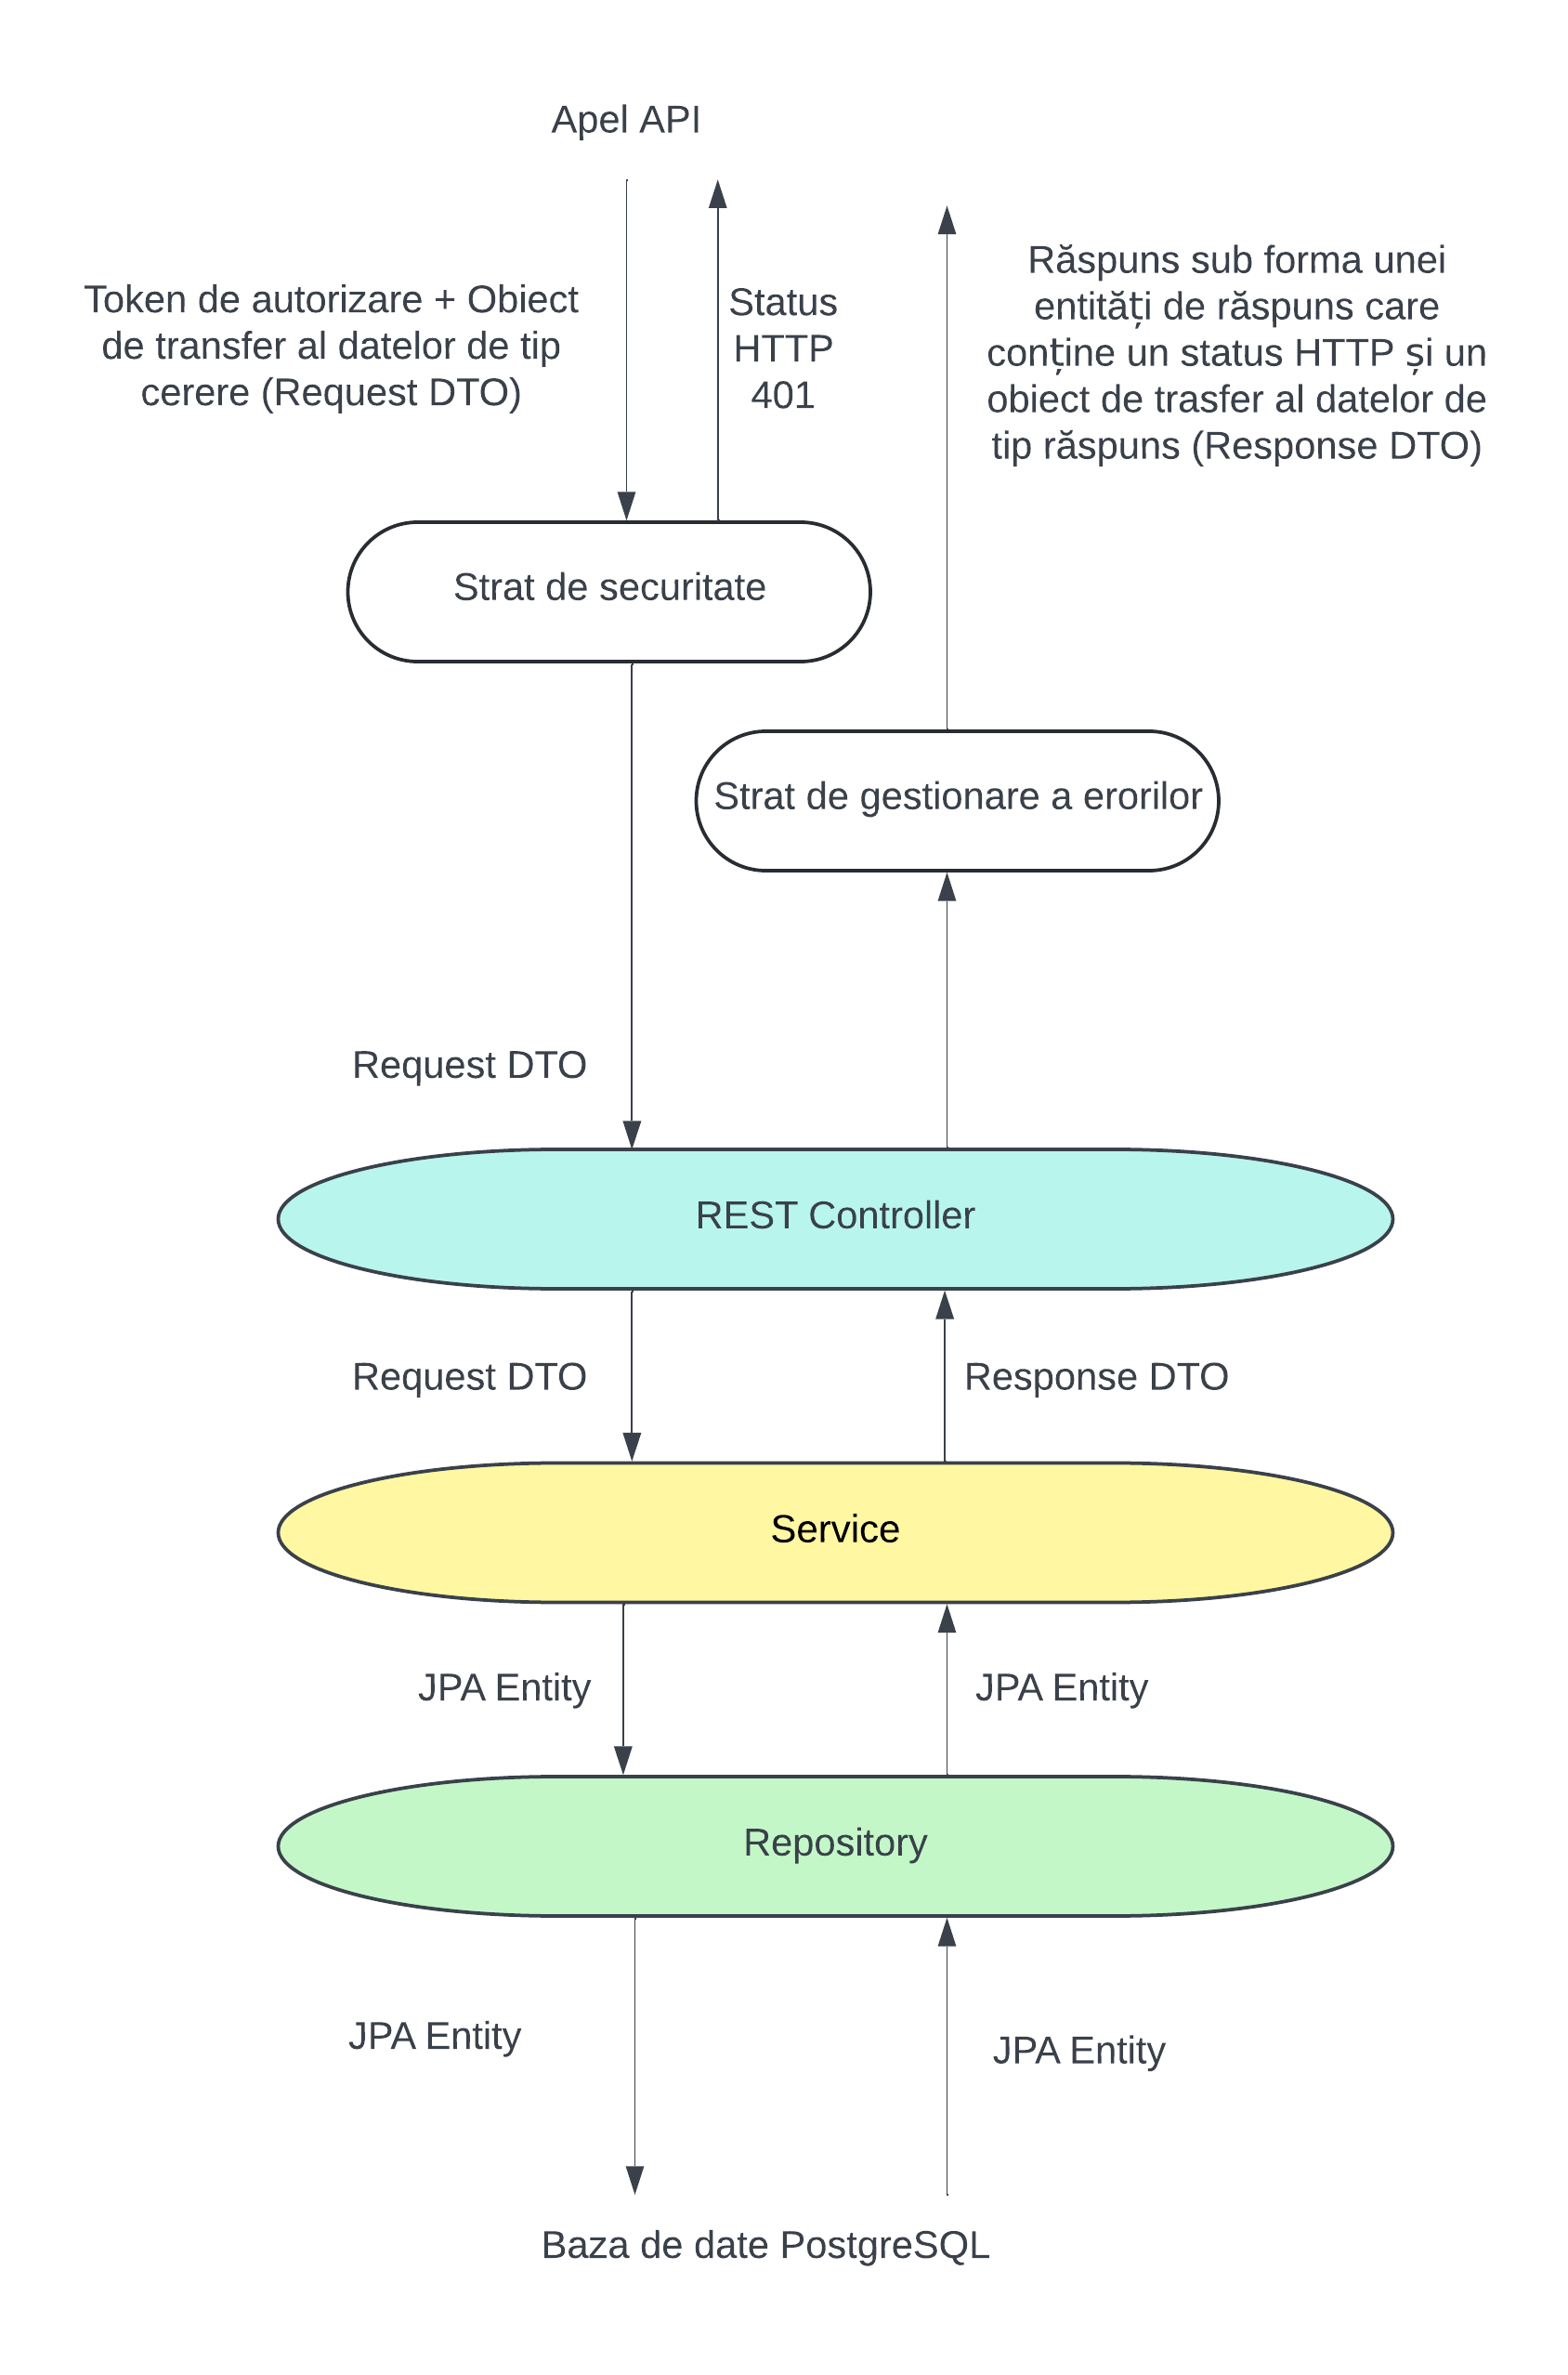
\includegraphics[width=0.6\linewidth]{controller-service-repository-flow.png}
	\caption{Fluxul datelor în componenta core}
	\label{controller-service-repository-flow}
 \end{figure}

Componenta care se ocupă cu funcționalitățile cele mai de bază ale aplicației este Taskage-Core. Aici se realizează operațiile CRUD asupra entităților și se gestionează cererile uzuale ale platformei. Structura componentei urmează patternul Controller-Service-Repository, popular în aplicațiile Spring Boot. Acest model de structurare a proiectului urmărește separarea sarcinilor unui sistem mare în părți mai ușor de manevrat. Fluxul datelor, reprezentat în figura \ref{controller-service-repository-flow}, este controlat, iar fiecare strat are un scop bine definit. 

Apelurile HTTP conțin un JWT token în header și trec prin filtrul de autorizare, implementat cu ajutorul Spring Securit. Dacă tokenul este aprobat ca fiind valabil și având criptat rolul corespunzător, apelul ajunge la end-point-ul asociat din controller. Altfel, aplicația intoarce un răspuns cu status HTTP 401(Unauthorized). Controllerele constituie API-ul aplicației și ca au ca unic scop expunerea unor funcționalități către agenți externi. Datele sunt primite sub forma unui obiect de transfer al datelor(Request DTO), care nu se traduce într-o entitate a bazei de date, fiind doar un mod de transmitere a informației între microservicii. Aceste DTO-uri trebuie de asemenea să respecte validările impuse câmpurilor prin Jakarta Validation.

Dacă DTO-ul a fost validat, acesta este trimis mai departe pentru procesare în zona cu logica de afaceri a aplicației, și anume serviciile. Serviciile procesează informația și eventual o mapează ca entități JPA spre a o transmite mai departe depozitelor(repositories). Depozitele reprezintă stratul de acces al datelor și se ocupă cu toate interacțiunile cu baza de date. Dacă totul se realizează cu succes, se va returna o entitate de răspuns cu statusul HTTP 200, eventual conținând un Response DTO cu datele cerute. Dacă se aruncă vreo excepție, aceasta va fi prinsă de clasa care se ocupă cu gestiunea erorilor la nivel global, GlobalExceptionHandler, și se va trimite înapoi un răspuns sugestiv.

\section{Taskage-DB}

Schema bazei de date este concepută pentru a stoca toate informațiile necesare gestionării unui proiect și generării de sugestii relevante. Urmărind o delimitare clară a responsabilităților, am identificat următoarele entități și relații(figura \ref{erd}):

 \begin{figure}[H]
	\centering
 	 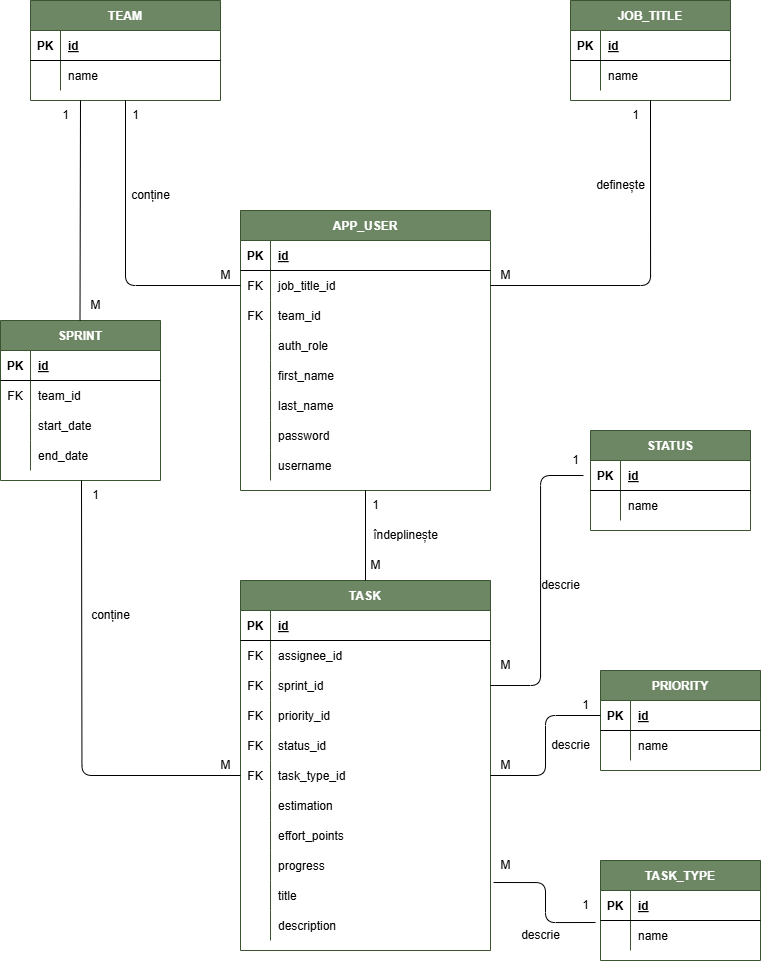
\includegraphics[width=1\linewidth]{ERD.png}
	\caption{Diagrama entitate-relație}
	\label{erd}
 \end{figure}

\begin{enumerate}
 	 \item \textbf{Team}(Echipă):
\begin{itemize}
\item[--] Atribute: id (PK), name
\item[--] Relații: App user(1:M), Sprint(1:M)
\item[--] Descriere: Reprezintă o echipă care lucrează la un proiect. Fiecare echipă are un id și un nume unice și o listă de utilizatori și sprinturi asociată.
\end{itemize}
	\item \textbf{Job title}(Poziție):
\begin{itemize}
\item[--] Atribute: id (PK), name
\item[--] Relații: App user(1:M)
\item[--] Descriere: Definește rolurile care se pot atribui în cadrul echipei. Fiecare rol poate fi asociat mai multor utilizatori. Fiecare înscriere a unui utilizator permite adăugarea unui nou rol.
\end{itemize}
	\item \textbf{App user}(Utilizator):
\begin{itemize}
\item[--] Atribute: id (PK), job_title_id (FK), team_id (FK), auth_role, first_name, last_name, password, username
\item[--] Relații: Team(M:1), Job title(M:1), Task(1:M)
\item[--] Descriere: Reprezintă un utilizator înregistrat în sistem de către administrator. Administratorul este adăugat o dată cu crearea bazei de date, făcând parte din „seed data”. Fiecare utilizator este asociat unei echipe, unui rol și se poate asocia mai multor sarcini de lucru.
\end{itemize}
	\item \textbf{Sprint}(Sprint):
\begin{itemize}
\item[--] Atribute: id (PK), team_id (FK), start_date, end_date
\item[--] Relații: Task(1:M), Team(M:1)
\item[--] Descriere: Reprezintă un sprint(unitate de timp în care membrii se angajează să livreze un set de funcționalități) din cadrul unui proiect. Fiecare sprint este legat de o echipă și poate conține mai multe sarcini de lucru.
\end{itemize}
	\item \textbf{Task}(Sarcină de lucru): 
\begin{itemize}
\item[--] Atribute: id (PK), assignee_id (FK), sprint_id (FK), priority_id (FK), status_id (FK), task_type_id (FK), estimation, effort_points, progress, title, description
\item[--] Relații: App user(M:1), Sprint(M:1), Priority(M:1), Status(M:1), Task type(M:1) 
\item[--] Descriere: Entitatea centrală, reprezentând sarcinile de lucru. Fiecare sarcină de lucru este asignată unui utilizator, unui sprint, și este descrisă de un status, o prioritate și un tip de task.
\end{itemize}
	\item \textbf{Status}(Status): 
\begin{itemize}
\item[--] Atribute: id (PK), name
\item[--] Relații: Task(1:M)
\item[--] Descriere: Definește statusurile posibile unei sarcini de lucru(tabelă dicționar).
\end{itemize}
	\item \textbf{Priority}(Prioritate): 
\begin{itemize}
\item[--] Atribute: id (PK), name
\item[--] Relații: Task(1:M)
\item[--] Descriere: Definește prioritățile posibile unei sarcini de lucru(tabelă dicționar).
\end{itemize}
	\item \textbf{Task type}(Tip de sarcină de lucru): 
\begin{itemize}
\item[--] Atribute: id (PK), name
\item[--] Relații: Task(1:M)
\item[--] Descriere: Definește tipurile posibile unei sarcini de lucru(tabelă dicționar).
\end{itemize}
\end{enumerate}

Fiecare tabel este normalizat pentru a preveni redundanța, iar multitudinea de tabele dicționar susține flexibilitatea și scalabilitatea. Varianta alternativă, salvarea dicționarelor în back-end prin intermediul tipului de date „enum”, presupune re-compilarea și re-deployerea aplicației pentru orice mică schimbare a cerințelor, în timp ce o modificare în baza de date este mult mai puțin costisitoare. De asemenea, construcția unui „enum” pentru etichetele folosite în interfața pentru utilizatori ar implica duplicarea datelor, ele trebuind declarate și în back-end și în front-end. În plus, legăturile definite de foreign keys asigură integritatea datelor, prevenind apariția de valori invalide.

Tabela „app_users” are câmpul special „auth_role” care poate lua una din valorile „ROLE_BASIC”(asociat membrilor normali ai unei echipe), „ROLE_MANAGER”(asociat managerilor echipelor) și „ROLE_ADMIN”(asociat administratorului paginii), urmând formatul înțeles de Spring Security. Speciale mai sunt tabelele de tip dicționar „priorities” și „statuses”, care nu implementează operații CRUD, ci servesc la stocarea unor date care altfel ar fi fost stocate în structuri de tip enum. Această alegere ajută la organizarea eficientă a codului și permite manevrarea mai ușoară a valorilor, putând fi chiar și actualizate la runtime.

\section{Taskage-Client}

Componenta care constituie front-end-ul aplicației este Taskage-Client. Aceasta este un proiect React care folosește MobX pentru gestionarea stării. Una din provocările principale la construcția unui proiect în React este lipsa de structură inerentă tehnologiei. Proiectele React nu au o structură de fișiere și un flux de date bine-definite, acestea rămânând responsabilitatea dezvoltatorului. Cele două mari abordări pentru structurarea aplicației sunt: abordarea orientată pe cateogorie și abordarea orientată spre funcționalitate. Prima variantă este mai puțin scalabilă, organizând fișierele după tipul lor(componente, pagini, modele) în timp ce a doua abordare rafinează mai departe structura, sortând componentele în funcție de funcționalitatea efectivă pe care o implementează. Din acest motiv am ales cea de-a doua alternativă.

 \begin{figure}[ht]
	\centering
 	 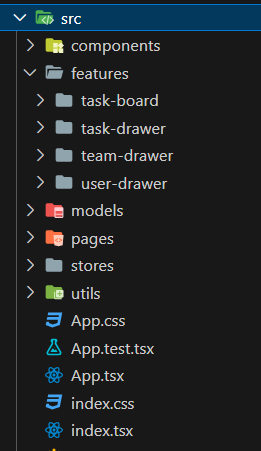
\includegraphics[width=0.3\linewidth]{FE-folder-structure.png}
	\caption{Structura de fișiere a aplicației React}
	\label{FE-folder-structure}
 \end{figure}

Deși front-end-ul reprezintă un SPA(Single Page Application), încărcarea paginilor se face pe baza rutelor pentru eficiență. Rutele sunt atât publice, cât și private. Cele private se pot accesa pe baza unor criterii precum tipul utilizatorului, iar în cazul lipsei privilegiilor de acces, acestea vor redirecționa utlizatorul către o pagină cu un mesaj sugestiv. Rutele servesc pagini, implementate în folderul „pages”, iar paginile randează diverse componente care, daca au logică complexă, sunt plasate într-un folder cu nume sugestiv funcționalității de care țin, în folderul „features”. Folderul „components” este rezervat pentru componente reutilizabile, generice. Stocarea datelor necesare în componente aflate la distanță mare pe ierarhia din DOM se face in „stores”, concept specific MobX. Tot aici se fac si apelurile către server și gestionarea datelor utilizatorului spre setarea corespunzătoare a tokenului în header-ul cererilor.

\section{Taskage-Helper}

Componenta care se ocupă cu analiza datelor stocate este Taskage-Helper. Aceasta este dezvoltată folosind Flask și comunică prin apeluri de API cu front-end-ul. Se observă faptul că este decuplată de celălalt serviciu de back-end, dezvoltarea sa putându-se realiza independent. Structura urmează o variantă adaptată a Controller-Service-Repository, în care filele sunt grupate în controllers, services și models, deoarece am ajuns la concluzia ca interacțiunea cu baza de date este prea simplă pentru a adăuga stratul de persistență. Operațiile de citire sunt executate direct din serviciile care au nevoie de datele respective. Terminologia Flask este destul de diferită de cea Spring Boot, astfel încât controllerele sunt numite „Blueprints” iar clasele care reprezintă entități ale bazei de date moștenesc clasa de bază „Model”.

Diagrama de secvență din figura \ref{sequence-diagram} reprezintă o expunere vizuală a interacțiunii dintre diferite componente ale aplicației, ca răspuns la acțiunea utilizatorului de click al butonului de cerere a sugestiei. Se observă clar fluxul controlat al informației într-o manieră abstractizată.

 \begin{figure}[H]
	\centering
 	 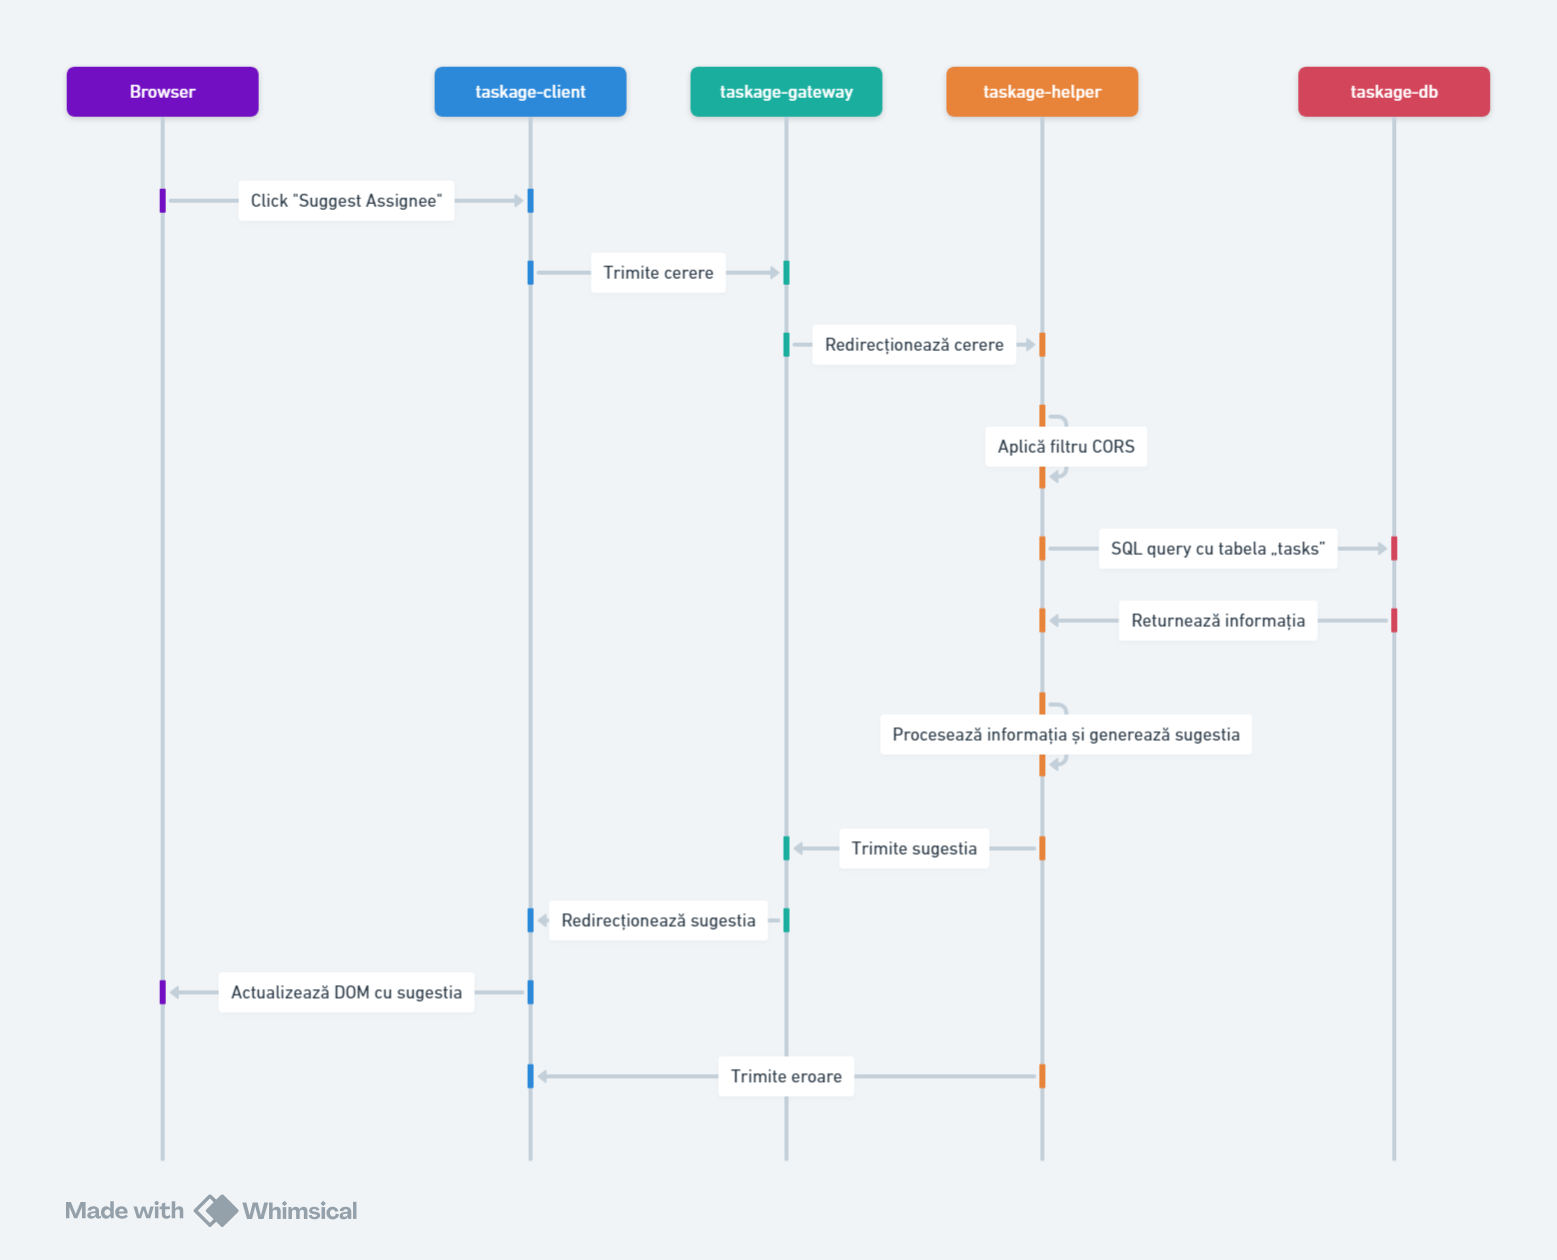
\includegraphics[width=1\linewidth]{sequence-diagram.png}
	\caption{Diagrama de secvență a Taskage-Helper}
	\label{sequence-diagram}
 \end{figure}
\chapter{Implementarea sistemului}

\section{Autentificare \& autorizare}\label{4-1}
Procesul de autentificare și autorizare este realizat pe baza unui JSON web token, care este validat la accesul majorității rutelor disponibile în aplicație, excepție făcând ruta „/login”. Această logică se desfășoară în felul următor:

\begin{itemize}

	\item Dacă utilizatorul nu are un token în spațiul de stocare local și încearcă să acceseze orice pagină în afară de cea de autentificare, atunci acesta este redirecționat către pagina de autentificare și își introduce numele de utilizator și parola sa. După o autentificare cu succes a utilizatorului, acesta primește înapoi un token, ce va fi stocat în browser, pe baza căruia își va autentifica și autoriza toate cererile.

	\item Dacă utilizatorul are un token în spațiul de stocare local, acesta este trimis odată cu cererea de accesare a unei pagini și token-ul este validat, atunci utilizatorul își păstrează accesul la pagini.
	
	\item Dacă utilizatorul are un token în spațiul de stocare local, iar acesta nu este valid din diverse motive, cum ar fi faptul că acesta a expirat, faptul că token-ul a fost semnat cu o cheie ce nu se potrivește cu cea utilizată pentru verificare sau pur și simplu acesta este malformat, atunci utilizatorul este redirecționat către pagina de autentificare și este nevoit să-și introducă din nou numele de utilizator și parola pentru a primi un nou token.

\end{itemize}

În plus, aplicația utilizează o serie de coduri de răspuns HTTP pentru diferitele scenarii explicate anterior, după cum se poate observa și din figura \ref{fig:authentication}, precum 200 atunci când token-ul este valid sau 401 atunci când acesta este invalid sau credențialele sunt greșite.

\begin{figure}[H]
	\centering
	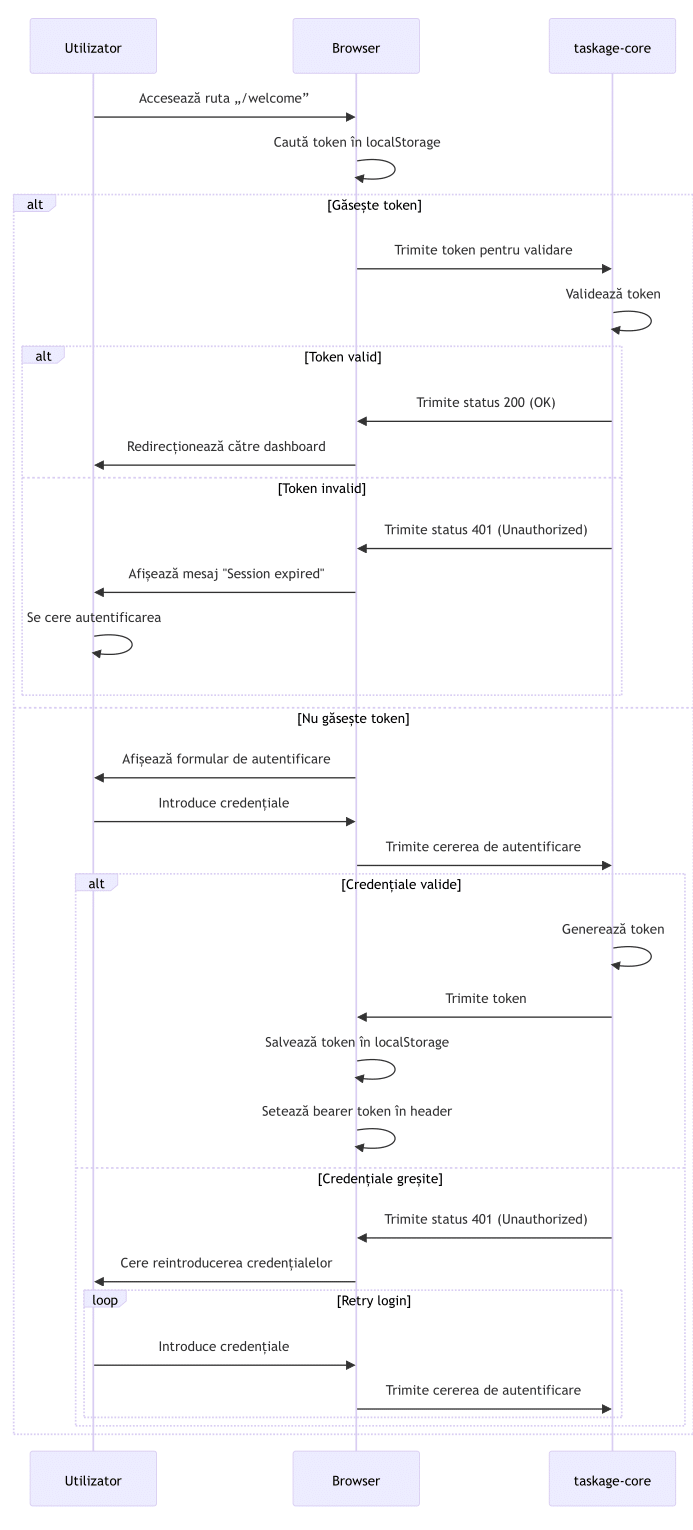
\includegraphics[width=0.6\linewidth]{seq-diagram-auth.png}
	\caption{Diagrama de secvență pentru autentificare}
	\label{fig:authentication}
\end{figure}

\section{Securitate}

Aplicația este securizată din mai multe perspective: Taskage-Client implementează o componentă personalizată de rută privată, endpoint-urile REST expuse de către componenta Taskage-Core, prin intermediul gateway-ului, sunt securizate utilizând modulul de securitate pus la dispoziție de către Spring, anume Spring Security, iar componenta Taskage-Helper este securizată prin pachetele specifice Flask.

Ruta privată a modulului front-end, utilizată în exemplul din în figura \ref{private-route-usage}, primește ca prop rolul care poate accesa ruta respectivă pentru a putea reutiliza componenta în contextul oricărui rol. Astfel, toți copiii din ierarhie, în cazul acesta rutele identificate prin constantele „TEAM_VIEW_ADMIN_LINK” și „USER_VIEW_ADMIN_LINK” vor fi protejați de logica rutei private.

\begin{figure}[H]
	\begin{lstlisting}[frame=single, style=java]
<Route element={<PrivateRoute allowedAuthRole={AUTH_ROLES.ADMIN} />} >
	<Route path={TEAM_VIEW_ADMIN_LINK} element={<TeamManager />} />
	<Route path={USER_VIEW_ADMIN_LINK} element={<EmployeeDirectory />} />
</Route>
	\end{lstlisting}
	\caption{Folosirea componentei PrivateRoute}
	\label{private-route-usage}
\end{figure}

Logica se poate observa în figura \ref{private-route}. Aceasta folosește un hook de tip „useEffect” pentru a detecta schimbarea paginii și a utilizatorului logat. Pentru oricare din aceste schimbări, încarcă un ecran de loading până verifică accesul, iar după ce metoda checkAccess determină asincron răspunsul, identifică dacă utilizatorul nu are acces la pagină fie pentru că acesta nu este logat, fie pentru că rolul său nu are dreptul pentru accesarea paginii respective. Dacă accesul este oferit, se poate încărca un „outlet”.

Outlet-ul reprezintă o componentă specifică React Router, ce ajută în dezvoltarea aplicațiilor ce implică rute imbricate. Acesta permite flexibilitatea unor componente modulare, ce pot fi incluse în cadrul aplicației, fapt dorit în cadrul aplicațiilor de tip SPA, ce ajută performanța, ridicând viteza cu care codul JavaScript este încărcat în browser-ul clientului, acesta din urmă nefiind nevoit să reîncarce toată pagina, ci doar o parte specifică. 

În cazul de față, utilizatorul este redirecționat către o pagină cu un mesaj sugestiv, după cum se poate observa în figura \ref{not-authenticated}, ce înștiințează utilizatorul cu privire la faptul ca nu este autentificat și, deci, nu are acces la conținuturile rutei accesate.

\begin{figure}[H]
	\begin{lstlisting}[frame=single, style=java]
	const PrivateRoute = observer(
	  ({ allowedAuthRole }: { allowedAuthRole: String }) => {
	    const location = useLocation();
	    const [isAllowed, setIsAllowed] = useState(false);
	    const [loading, setLoading] = useState(true);
	    const [navigateToRoute, setNavigateToRoute] = useState<string>("");
	
	    useEffect(() => {
	      const checkAccess = async () => {
	        if (userStore.currentUser) {
	          const currentUser = userStore.currentUser;
	          if (currentUser.user.authRole === allowedAuthRole) {
	            setIsAllowed(true);
	          } else {
	            setNavigateToRoute(UNAUTHORIZED_ACCESS_LINK);
	          }
	        } else {
	          setNavigateToRoute(NOT_AUTHENTICATED_LINK);
	        }
	        setLoading(false);
	      };
	
	      checkAccess();
	    }, [userStore.currentUser, location]);
	
	    return loading ? (
	      <Spin />
	    ) : isAllowed ? (
	      <Outlet />
	    ) : (
	      <Navigate to={navigateToRoute} replace />
	    );
	  }
	);
	\end{lstlisting}
	\caption{Componenta PrivateRoute}
	\label{private-route}
\end{figure}

 \begin{figure}[ht]
	\centering
 	 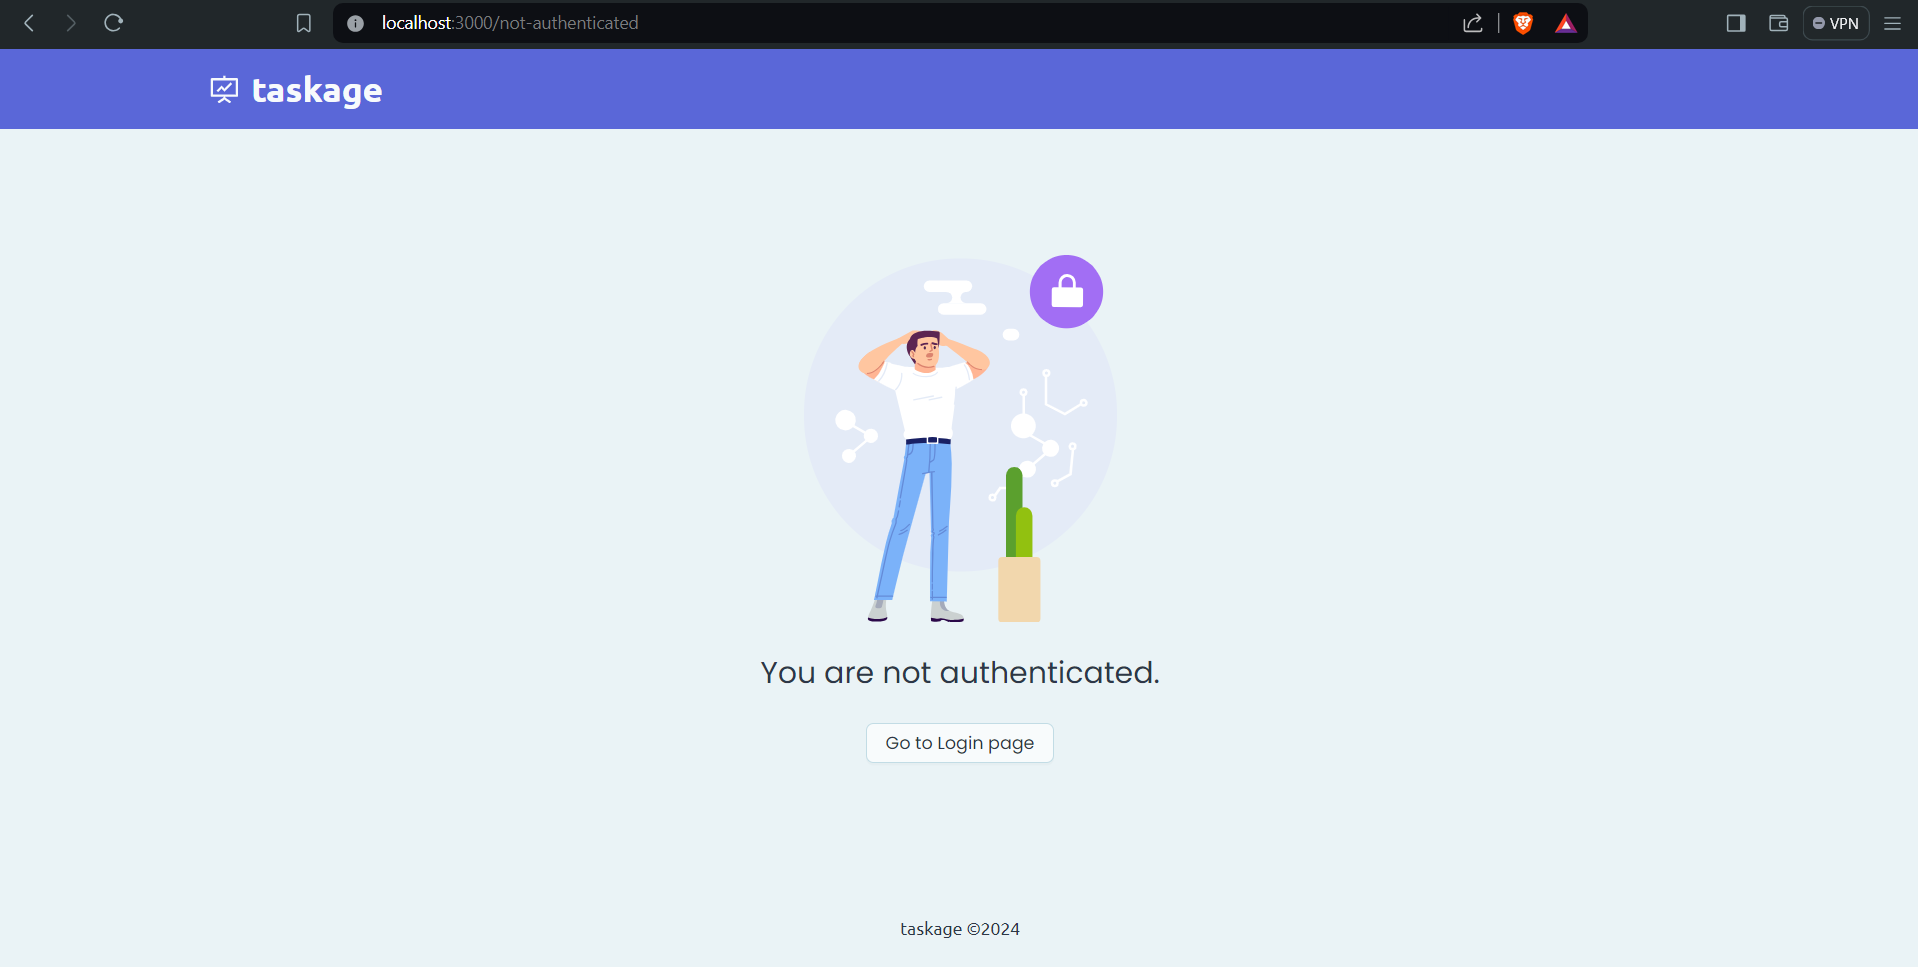
\includegraphics[width=1\linewidth]{not-authenticated.png}
	\caption{Pagina de redirecționare pentru utlilizatorii neautentificați}
	\label{not-authenticated}
 \end{figure}

Configurarea modulul Security al componentei Taskage-Core se află într-o clasa adnotată „@Configuration”, în cadrul căreia suprascriem metode precum „securityFilterChain”, „passwordEncoder” și „corsConfigurationSource”, pentru a configura gradul de securitate aplicat end-point-urilor REST. Adnotările facilitează munca dezvoltatorului, constiuind un mod de a asocia metadate diferitelor clase, pe care JVM-ul le va interpreta pentru compilare. „SecurityFilterChain” determină filtrarea securizată a cererilor pe baza token-ului, „passwordEncoder” criptează parolele înainte de salvarea în baza de date, iar „corsConfigurationService” limiteză accesul cross-origin pentru a bloca cererile care vin de pe IP-uri care nu corespund clientului nostru.

Fluxul autentificării și autorizării este definit în figura \ref{authentication-flow}. În urma conectării cu succes al unui utilizator, pe bază de nume de utilizator și parolă, componenta Taskage-Core eliberează un JSON Web Token (JWT), pe baza căruia cererile HTTP făcute ulterior de către client pot fi autorizate. Mai exact, în urma autentificării cu succes a utilizatorului se va crea un JWT, semnat de către aplicație cu ajutorul algoritmului HS512(un algoritm simetric, specific situațiilor în care cel care semnează tokenul este și cel care îl va verifica), căruia îi sunt atașate rolurile utilizatorului autentificat. Un astfel de rol este de forma „ROLE_[nume_rol]”, unde [nume_rol] poate fi orice denumire aleasă, însă, în cadrul proiectului avem trei tipuri de utilizatori: „ROLE_BASIC”(asociat membrilor normali ai unei echipe), „ROLE_MANAGER”(asociat managerilor echipelor) și „ROLE_ADMIN”(asociat administratorului paginii), fiecare având stocat în baza de date propriile privilegii și permisiuni, sub formă de roluri.

În plus, JWT-ul eliberat de către serviciul Spring are și o perioadă predefinită de existență („time to live”), configurat la compilare, iar tokenul de autorizare și datele utilizatorului curent sunt stocate în localstorage-ul browserului spre autentificarea automată. După părăsirea paginii, la o nouă accesare, se verifica dacă credențialele se află în localStorage și dacă token-ul este încă valid, print-un apel suplimentar către backend care decriptează token-ul și verifică time to live-ul setat anterior.

 \begin{figure}[H]
	\centering
 	 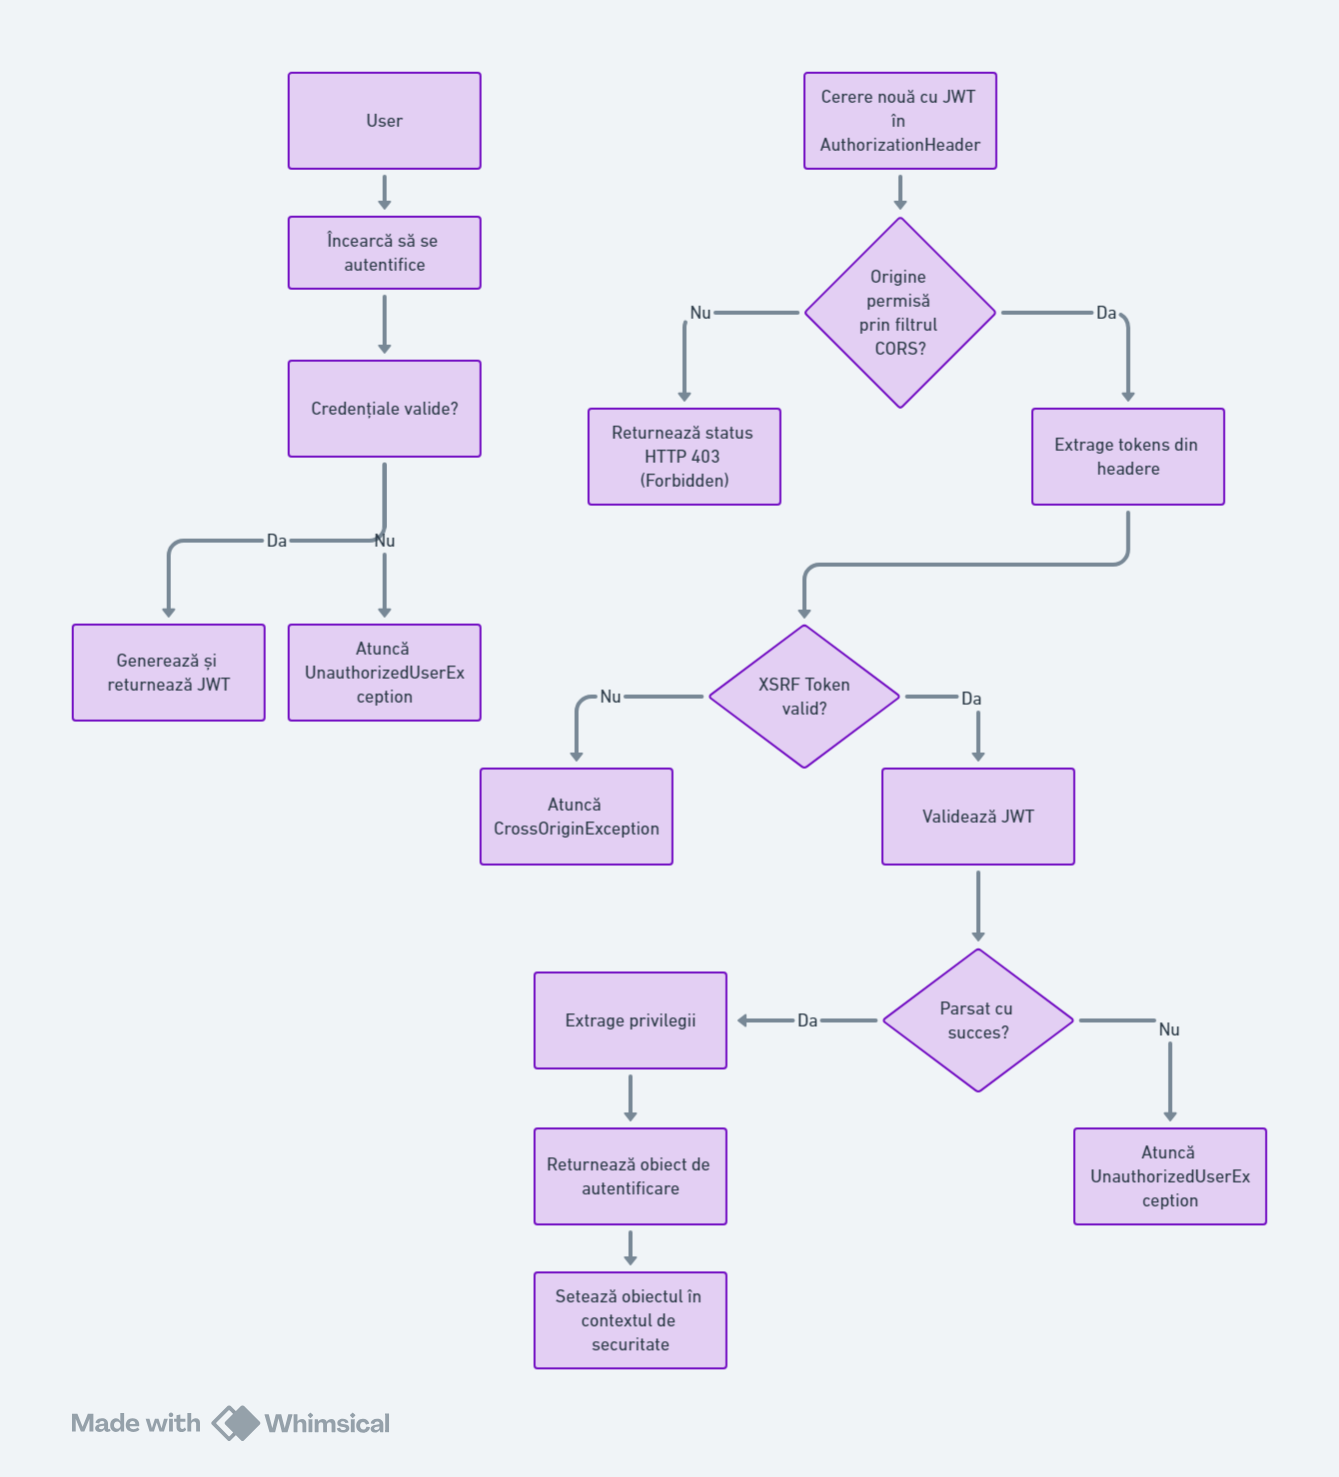
\includegraphics[width=1\linewidth]{security-flowchart.png}
	\caption{Fluxul autentificării și autorizării}
	\label{authentication-flow}
 \end{figure}

\section{Gestionarea excepțiilor}

Pentru a crește stabilitatea aplicației și a gestiona excepțiile care apar inevitabil în timpul folosirii, am implementat un strat în plus de siguranță prin crearea unei clase de gestionare a excepțiilor, care permite prinderea lor din contextul întregii aplicații și întoarcerea unui raspuns explicit clientului legat de problema întâmpinată. Pentru aceasta, am folosit adnotarea „@ControllerAdvice”, care transformă clasa într-un interceptor de excepții, pentru a fi nevoie de gestionarea excepțiilor în fiecare controller individual.

În cadrul clasei astfel definite putem explicita metoda de gestionare a fiecărei excepții care poate fi aruncată. În figura 4.6 se observă un astfel de exemplu, unde excepția este generică, dar este invocată cu un mesaj care va fi întors cu statusul explicit de către endpoint.

\begin{figure}[H]
	\begin{lstlisting}[frame=single, style=java]
@ControllerAdvice
public class GlobalExceptionHandler {
    @ExceptionHandler(NotFoundException.class)
    public ResponseEntity<String> handleNotFoundException(NotFoundException e) {
        return ResponseEntity.status(HttpStatus.NOT_FOUND).body(e.getMessage());
    }
	\end{lstlisting}
	\label{not-found-exception}
	\caption{Gestionarea excepției NotFoundException}
\end{figure}

La celălalt capăt, în componenta front-end, am identificat aceste erori și am afișat o notificare legat de problema întâmpinată. Conceptul de permisiuni din JS permite indicarea de acțiuni de executat după comanda asincronă prin metodele .then() si .catch(), așa cum apare în figura 4.7.

\begin{figure}[H]
	\begin{lstlisting}[frame=single, style=java]
create = (newTask: Task, teamId: number) => {
  axios
    .post(`${TASKS_API_URL}/create`, newTask)
    .then(() => {
      sprintStore.getAllForTeam(teamId);
      message.success("Task added successfully");
    })
    .catch((err: AxiosError) => {
      handleAxiosError(err);
      });
  };
	\end{lstlisting}
	\label{http-status}
	\caption{Gestionarea statusurilor HTTP în client }
\end{figure}


\section{Persistență}

Atât crearea schemei bazei de date, cât și interacțiunea cu baza de date, s-au realizat prin ORM-ul (Object Relational Mapping) oferit de Spring, anume Spring JPA (Jakarta Persistence API). Am optat pentru această opțiune prin configurarea specifică Hibernate, unde ddl-auto poate fi setat pentru transformarea automată a modelelor adnontate „@Entity” în scripturi SQL.

În zona de back-end, Spring JPA oferă un nivel de abstractizare peste stratul de SQL, permițând crearea de tabele, relații și constrângeri prin adnotări, precum „@Entity” pentru a semnala că această clasă reprezintă de fapt un model pentru tabela din baza de date, „@Id” pentru a semnala că un câmp dintr-o clasă asociată unei tabele este cheie primară și altele asemenea. Spring JPA ne oferă posibilitatea de a seta algoritm de generare automată a cheilor primare, de a crea coloane read-only, de a adăuga constrângeri atât banale, precum nullable și unique, cât și constrângeri relaționale precum „@OneToMany”. Codul SQL în dialectul specific, în cazul acesta PostgreSQL, poate fi vizualizat după inițializarea bazei de date:

\begin{figure}[H]
	\begin{lstlisting}[frame=single, style=yaml]
-- auto-generated definition
create table tasks
(
    assignee_id   integer
        constraint fkrwm5ssj09it2xfnlobqo3fk9x
            references app_users,
    effort_points integer,
    estimation    integer,
    id            serial
        primary key,
    priority_id   integer,
    progress      integer,
    sprint_id     integer
        constraint fkl5ac6kwptw5o73haren9qnkav
            references sprints,
    status_id     integer,
    task_type_id  integer
        constraint fkkb5gyrxp5x7p5inusg3ykdugt
            references task_types,
    description   varchar(255),
    title         varchar(255)
);

alter table tasks
    owner to postgres;
	\end{lstlisting}
	\label{http-status}
	\caption{ Cod PostgreSQL auto-generat }
\end{figure}

Un alt avantaj este specificarea metodei de aducere a datelor, care poate fi LAZY sau EAGER. În varianta LAZY, datele date de relațiile obiectului nu sunt încărcate decât la apelarea unui getter, în schimb ce varianta EAGER recuperează din start toate datele. Având în vedere că lucrăm cu o aplicație web, de ajutor mai este adnotarea „@JsonIgnore” care ne permite să manipulăm forma obiectului trimis prin HTTP. Aceasta este de multe ori necesară, pentru că reprezentarea relațiilor nu se face prin chei externe, ci prin referințe la obiectele care se află în relație, iar trimiterea acestora ca răspuns HTTP poate genera referințe circulare.

Mai departe, interacțiunea cu baza de date este simplificată, fiind mai prietenoasă cu utilizatorul decât standardul Java. În varianta standard, se folosește clasa JDBCTemplate, prin intermediul căreia ai scrie SQL nativ. În schimb, utilzând JPA, procesul este vast simplificat, având ca premise doar crearea unei interfețe ce derivează una deja existentă, generică, anume JpaRepository<TIP, TIP_ID>. 

În cadrul acestei metode, Spring JPA permite definirea de metode doar descriind acțiunea necesară. Spre exemplu, pentru a găsi toți utilizatorii dintr-o echipă anume, am putea specifica o metodă cu o signatură precum: „findAllByTeam(String)”, iar implementarea ar fi rezolvată de către ORM-ul utilizat, astfel, oferind una dintre cele mai prietenoase API-uri pentru a interacționa cu baza de date.

\section{Actualizări în timp real}

Actualizările în timp real sunt asigurate prin WebSockets. Aceștia sunt canale bidirecționale de comunicare, care funcționează pe baza unei conexiuni stabilite printr-un handshake între client și server. Într-o conexiune HTTP clasică, sunt necesare cereri repetate din partea clientului pentru a primi date de la server. Problemele cauzate sunt clare: server-ul este obligat să deschidă numeroase conexiuni TCP pentru fiecare client(unul pentru primirea datelor și unul pentru transmiterea datelor), iar clientul este forțat să țină scorul cererilor și conexiunilor pentru a corela răspunsurile.  Aceste probleme sunt rezolvate prin WebSockets, prin care cele două componente își pot trimite date fără aceste constrângeri. Din acest motiv, WebSockets sunt de ajutor pentru actualizările în timp real, fiind folosiți în aplicații precum aplicațiile de mesagerie sau jocurile multiplayer\cite{websockets-protocol}.

Pentru implementare am folosit clasicul WebSocket pus la dispoziție de JavaScript, creând clasa WebSocketService pentru gestionarea ciclului de viata a fiecărui socket, unde sunt definite event handler-ele pentru deschiderea conexiunii, primirea mesajelor și închiderea conexiunii. Am utilizat acest serviciu în cadrul store-urilor MobX, precum se poate observa în exemplul din figura \ref{websocket-reaction}. Aici am definit un reaction, concept specific MobX, ce funcționează ca un listener ce așteaptă modificarea valorii returnate de o metodă și declanșează o altă metodă ca răspuns. În acest caz, am vrut ca la autentificarea si log out-ul unui utilizator să se deschidă, respectiv închidă conexiunea, dar la deschidere să definim acțiunile și modul lor de gestionare.

\begin{figure}[H]
	\begin{lstlisting}[frame=single, style=java]
  constructor() {
	//...
    reaction(
      () => userStore.isSignedIn,
      (isLoggedIn) => {
        if (isLoggedIn) { this.connectWebSocket(); }
        else { this.disconnectWebSocket(); } }
    ); } }

  connectWebSocket = () => {
    WebSocketService.connect();
    WebSocketService.on("ADD", this.handleWebSocketMessage);
    // ... idem pentru update și delete };

  disconnectWebSocket = () => {
    WebSocketService.disconnect();
    WebSocketService.off("ADD");
    // ... idem pentru update și delete };

  updateTeamsFromWebSocket = (message: any) => {
    const { action, newTeam, teamId } = message;
    switch (action) {
      case "ADD":
        this.allTeams = this.allTeams.concat(newTeam);
        break;
      case "UPDATE":
        this.allTeams = this.allTeams.map((team) => (team.id === newTeam.id ? newTeam : team));
        break;
      case "DELETE":
        this.allTeams = this.allTeams.filter((team) => team.id !== teamId);
        break;
      default:
        break;
    } };

  handleWebSocketMessage = (message: any) => {
    this.updateTeamsFromWebSocket(message); };
	\end{lstlisting}
	\label{websocket-reaction}
	\caption{ Integrarea serviciului WebSocketService în TeamStore }
\end{figure}

Pe partea serverului, am folosit WebSockets puși la dispoziție de Spring. Aceasta a necesitat definirea unor handlers și înregistrarea lor pe diferitele rute pe care se va stabili conexiunea. Acești handleri au fost folosiți în servicii pentru ca, după efectuarea operațiilor cerute, informația nouă să fie propagată către toate sesiunile deschise.

\section{Algoritm de analiză al datelor}

Componenta Taskage-Helper are ca unic rol prelucrarea datelor stocate referitor la sarcinile de lucru. Am identificat 3 informații importante referitoare la taskuri: punctele de efort hotărâte de echipă, ce indică complexitatea, prioritatea, ce indică cât de urgentă este rezolvarea sa, și tipul, ce indică domeniul de cunoștințe folositor la indeplinirea lui(arbitrare, fiecare echipă își poate stabili propriile categorii de taskuri).

Am creat un API care primește aceste trei informații referitoare la un task și id-ul echipei în cadrul căreia e adăugat și caută să găsească persoana cea mai potrivită pentru a îl duce la capăt. O astfel de persoană este, probabil, o persoană care a mai realizat taskuri asemănătoare, iar dacă aceste taskuri sunt uzuale în echipă, membrul pentru care taskurile de acest gen sunt principale. Totuși, cele trei informații aflate la dispoziție sunt destul de diferite. Primele două sunt scalare, reprezintă metrici de evaluare ori a priorității, ori a dificultății, măsurate la rândul lor pe scări diferite, iar ultima informație, tipul de task, este o simplă etichetă reprezentată arbitrar printr-un număr. Toate acestea indică faptul că ele ar trebui tratate diferit.

Algoritmul aduce din baza de date toate informațiile curente despre taskuri realizate de echipa în cauză și calculează câte un scor de familiaritate pentru fiecare membru al echipei. Scorul este calculat ca media similarității dintre fiecare task realizat de acesta și task-ul nou, iar membrul cel mai potrivit va fi cel care a realizat, per total, cele mai similare task-uri, urmând să se țină cont și de capacitatea sa în sprintul curent.

Am menționat că două dintre detaliile referitoare la task vor fi tratate diferit de ultimul, pe baza faptului că însemnătatea este altfel interpretată. Astfel, am ales ca metode de calcul similaritatea cosinuisoidală și coeficientul Jaccard de similaritate.

Datele sunt întoarse din baza de date în tupluri de assignee_id și detalii despre task, sub forma unui array format din priority_id, effort_points și task_type_id. Primele două, având în vedere descrierea anterioară, sunt tratate separat și sunt inițial normalizate folosind MinMaxScaler din biblioteca scikit-learn. Acesta încadrează valorile uniform în intervalul [0, 1] pentru a asigura faptul că nicio caracteristică nu o să influențeze mai mult decât celelalte rezultatul.

Similaritatea cosinusoidală măsoară cosinusul unghiului dintre doi vectori, pe baza formulei: 

\[
\text{cosine_similarity} = \frac{A \cdot B}{\|A\| \|B\|}
\]

unde numărătorul este produsul scalar al vectorilor, iar numitorul este dat de produsul lungimilor vectorilor. Prin această împărțire, produsul scalar este normalizat, iar similaritatea este calculată strict pe baza direcției. Aceasta este de folos într-un context în care valorile pot varia considerabil, având în vedere că o sarcină de lucru ce necesită mult efort dar nu are prioritate mare poate să fie similară unei alte sarcini de lucru cu valori diferite, dar direct proporționale.

Coeficientul de similaritate Jaccard este folosit pentru a compara atribute categorice(etichete) și este definit ca raportul dintre cardinalul întersecției și cardinalul reuniunii a două mulțimi, rezultând formula:

\[
\text{jaccard_similarity} = \frac{|A \cap B|}{|A \cup B|}
\]


Acest coeficient măsoară similaritatea în termeni de elemente comune și este, uzual, folosită pentru date non-numerice. În cazul nostru, etichetele ce indică tipul taskurilor(de exemplu „Development” sau „Testing”) nu au o ordine naturală, deci nu putem măsura distanțe. Astfel, coeficientul Jaccard caută prezența sau absența elementelor, mai degrabă decât valorile lor. În plus, este ușor adaptabil cazurilor în care o nouă categorie este introdusă, nefiind nevoie de readaptarea algoritmului.
\chapter{Utilizarea aplicației și funcționalități}

\section{Prezentarea interfeței}

Ruta implictă, la accesarea aplicației, este „/login”. În figurile \ref{fig:taskage-login}\ și \ref{fig:taskage-login-auto} este prezentată interfața încărcată ca răspuns, în cele două contexte posibile: autentificare explicită și autentificare automată. Aceste pagini sunt rezultatul procesului complex care se declanșează la accesarea rutei „/login”, proces descris în secțiunea 4.1.

În cazul în care browser-ul nu conține în local storage un token de autentificare, sau token-ul găsit este expirat, este afișat un formular de autentificare. Aici, utilizatorul trebuie să introducă credențialele primite de la administrator, singurul tip de utilizator care are privilegiul creării conturilor. Datele sunt preluate din formular și trimise către componenta Taskage-Core, iar răspunsul este transformat într-un toast explicit cu feedback legat de succesul acțiunii. 

 \begin{figure}[H]
	\centering
 	 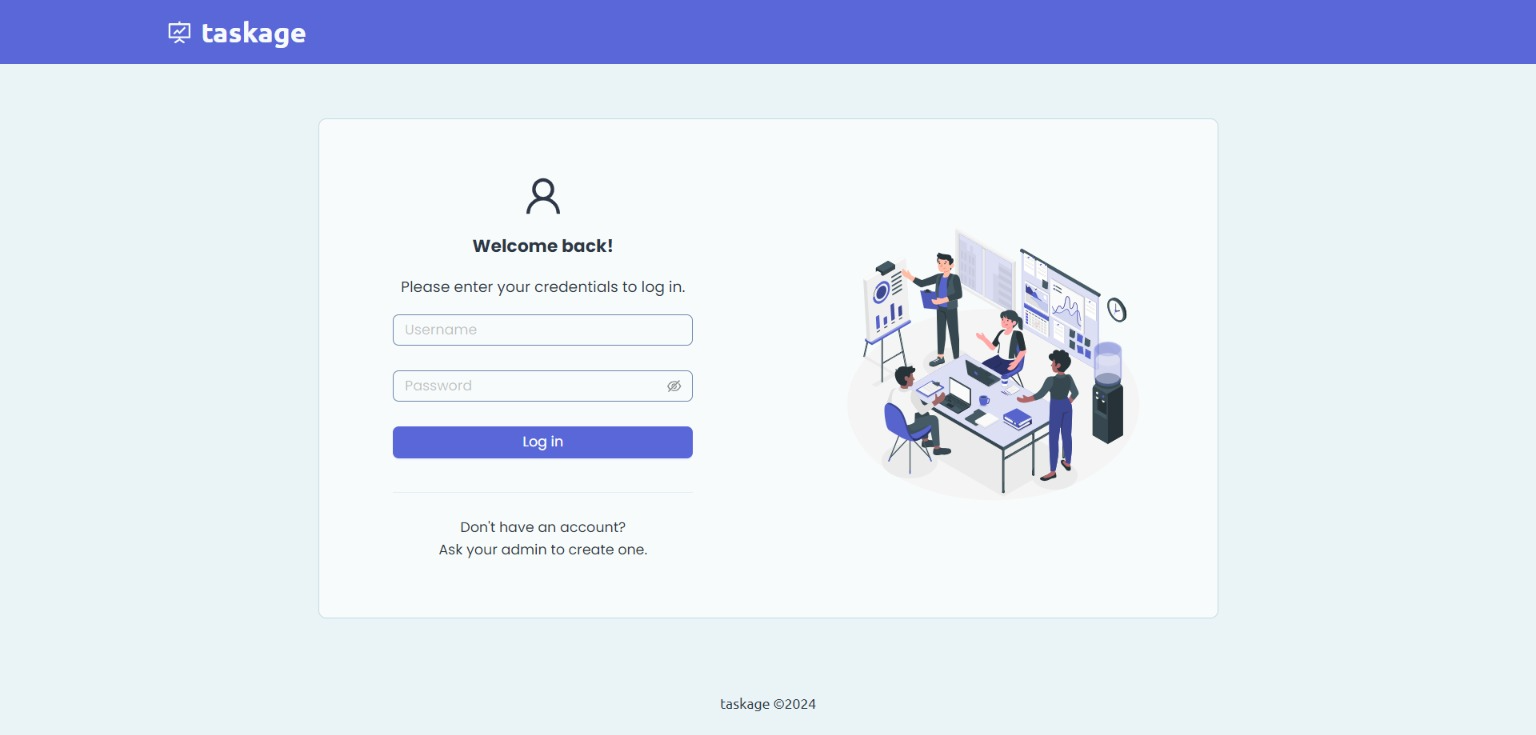
\includegraphics[width=\linewidth]{taskage-login.png}
	\caption{Pagina încărcată de ruta „/login” fără autentificare automată}
	\label{fig:taskage-login}
 \end{figure}

Ca urmare a autentificării explicite, în proprietatea localStorage a browser-ului se salvează un obiect numit „authenticated-user”, care conține atât datele utilizatorului cât și token-ul de acces al acestuia(figura \ref{fig:taskage-login-auto}).

 \begin{figure}[H]
	\centering
 	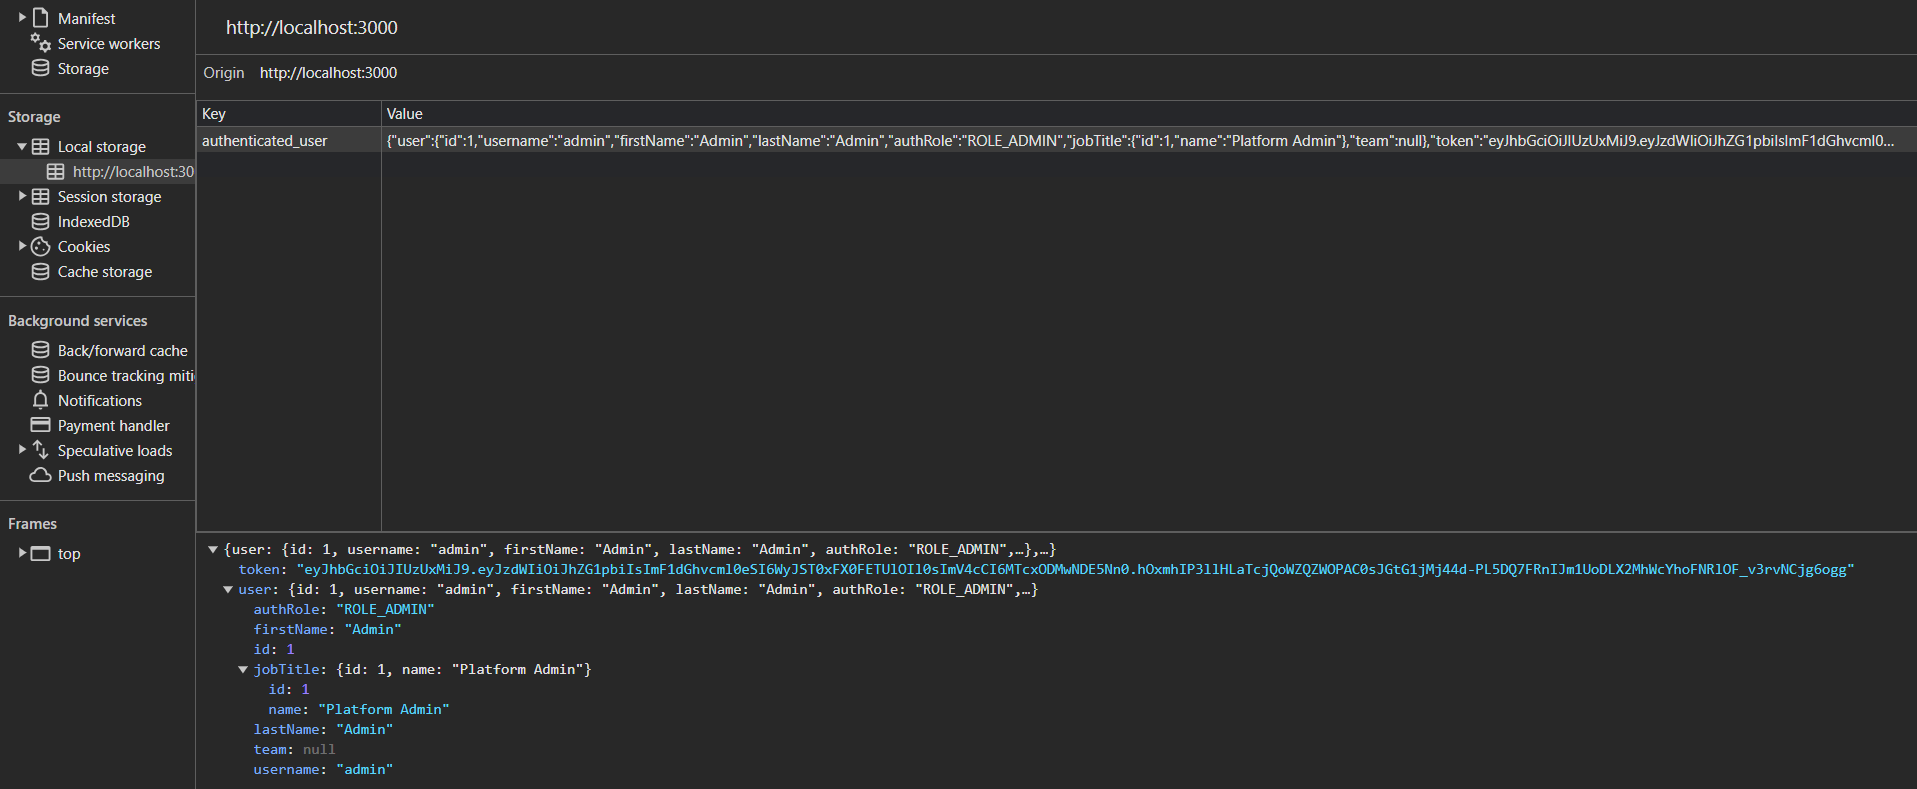
\includegraphics[width=\linewidth]{localstorage-token.png}
	\caption{Obiectul salvat în localStorage după autentificare}
	\label{fig:token}
 \end{figure}

Atunci când browser-ul conține în localStorage un token care nu a expirat, se realizează autentificarea automată, iar utilizatorul este redirecționat către propriul panou de control și primește un toast sugestiv, așa cum apare în a doua captură de ecran(figura \ref{fig:taskage-login-auto}). De asemenea, acesta este anunțat printr-o notificare de faptul că autentificarea s-a realizat automat și poate să se deconecteze explicit prin butonul „Log Out”, prezent în header.

 \begin{figure}[H]
	\centering
 	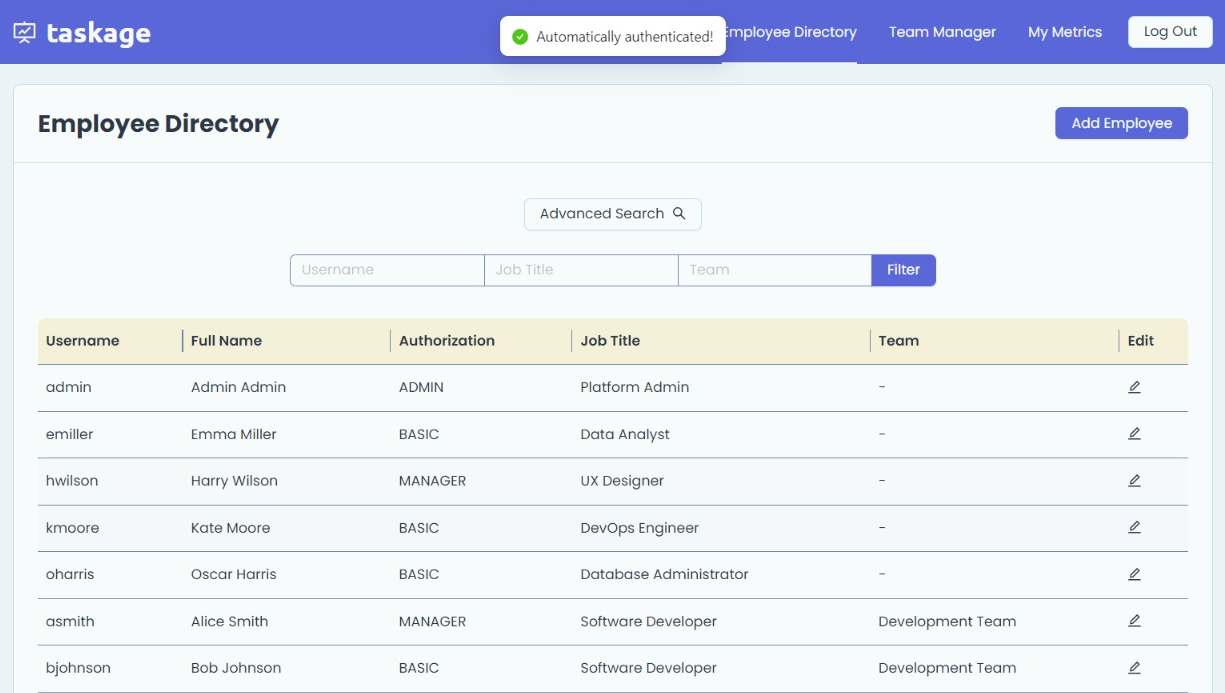
\includegraphics[width=\linewidth]{taskage-login-redirect-1.png}
	\caption{Pagina răspuns în urma autentificării automate}
	\label{fig:taskage-login-auto}
 \end{figure}

Paleta de culori este setată asupra componentelor Ant Design prin intermediul componentei „ConfigProvider”, care pune la dispoziție prop-ul „theme”. Aici, tema de culori poate fi indicată prin cheia „components”, care aplică stilul pe componente specifice ale bibliotecii, sau „tokens”, care aplică stilul prin etichetele indicați în documentație ca fiind asociate anumitor componente.

Mai departe, fluxul utilizării aplicației depinde de tipul de utilizator(BASIC, MANAGER sau ADMIN) care s-a autentificat, diferențiere făcută prin token-ul de autorizare, generat anterior, acum trimis ca Authorization header pentru fiecare request(figura \ref{fig:auth-token}).

 \begin{figure}[H]
	\centering
 	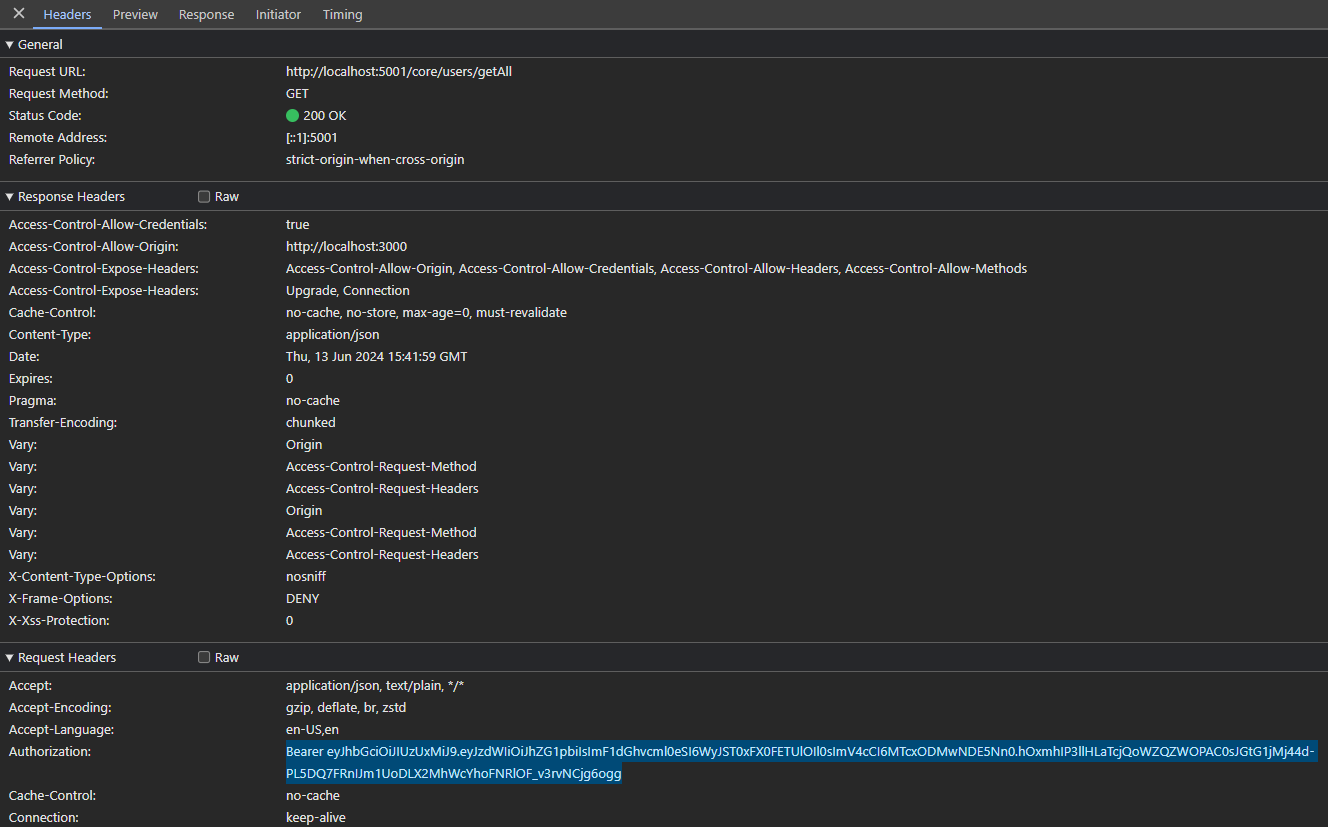
\includegraphics[width=\linewidth]{auth-token.png}
	\caption{Authorization header într-o cerere HTTP de administrator}
	\label{fig:auth-token}
 \end{figure}

\section{Funcționalitățile rolului de administrator}

Reprezentative pentru identitatea vizuală a aplicației sunt panourile de control ale administratorului, care poate accesa „Employee Directory” și „Team Manager”. Acestea se folosesc de componente reutilizabile pentru încărcarea componentei de căutare avansată și de pentru diversele formulare.

Pagina „Employee Directory” este cea încărcată default la conectarea administratorului, așa cum s-a prezentat anterior. Această pagină este compusă dintr-un tabel paginat, ce conține intrări cu toți angajații înregistrați la momentul respectiv pe platformă. Mai mult, prin intermediul unui sistem de filtrare pe bază de nume de utilizator, poziție, sau echipă, este facilitată căutarea unui angajat pentru administratori(figura \ref{fig:filter-employee}).

 \begin{figure}[H]
	\centering
 	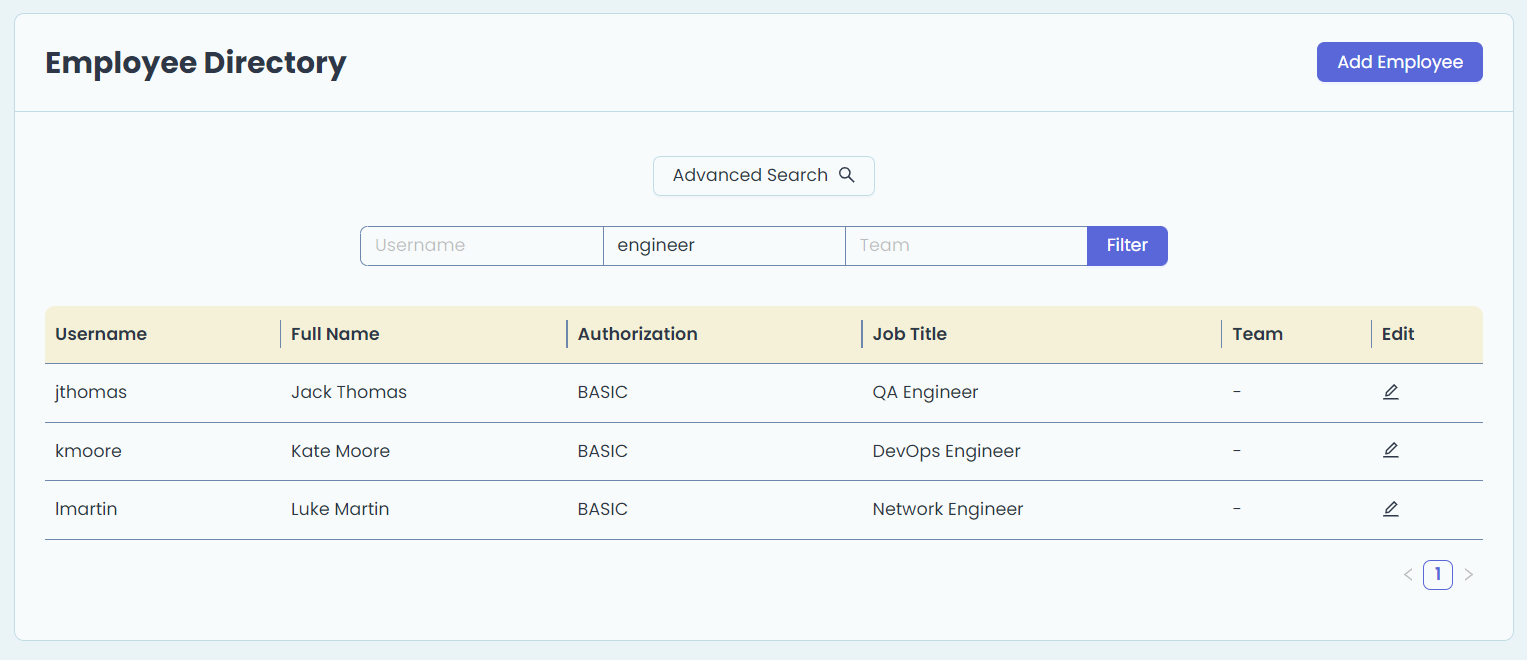
\includegraphics[width=\linewidth]{filter-employee.png}
	\caption{Rezultatul filtrării după titulatura „engineer”}
	\label{fig:filter-employee}
 \end{figure}

În plus, există funcționalități de adăugare a unui angajat nou, editarea a detaliilor privind oricare dintre angajații de pe platformă, sau ștergere a angajaților. Acestea se realizează printr-un formular generic care se randează sub două moduri, cel de creare și cel de editare(figurile \ref{fig:user-form-create} și \ref{fig:user-form-update}).

Formularul de creare a unui cont de utilizator cere introducerea tuturor datelor necesare identificării acestuia, câmpurile fiind validate înainte de trimiterea cererii către back-end.

 \begin{figure}[H]
	\centering
 	 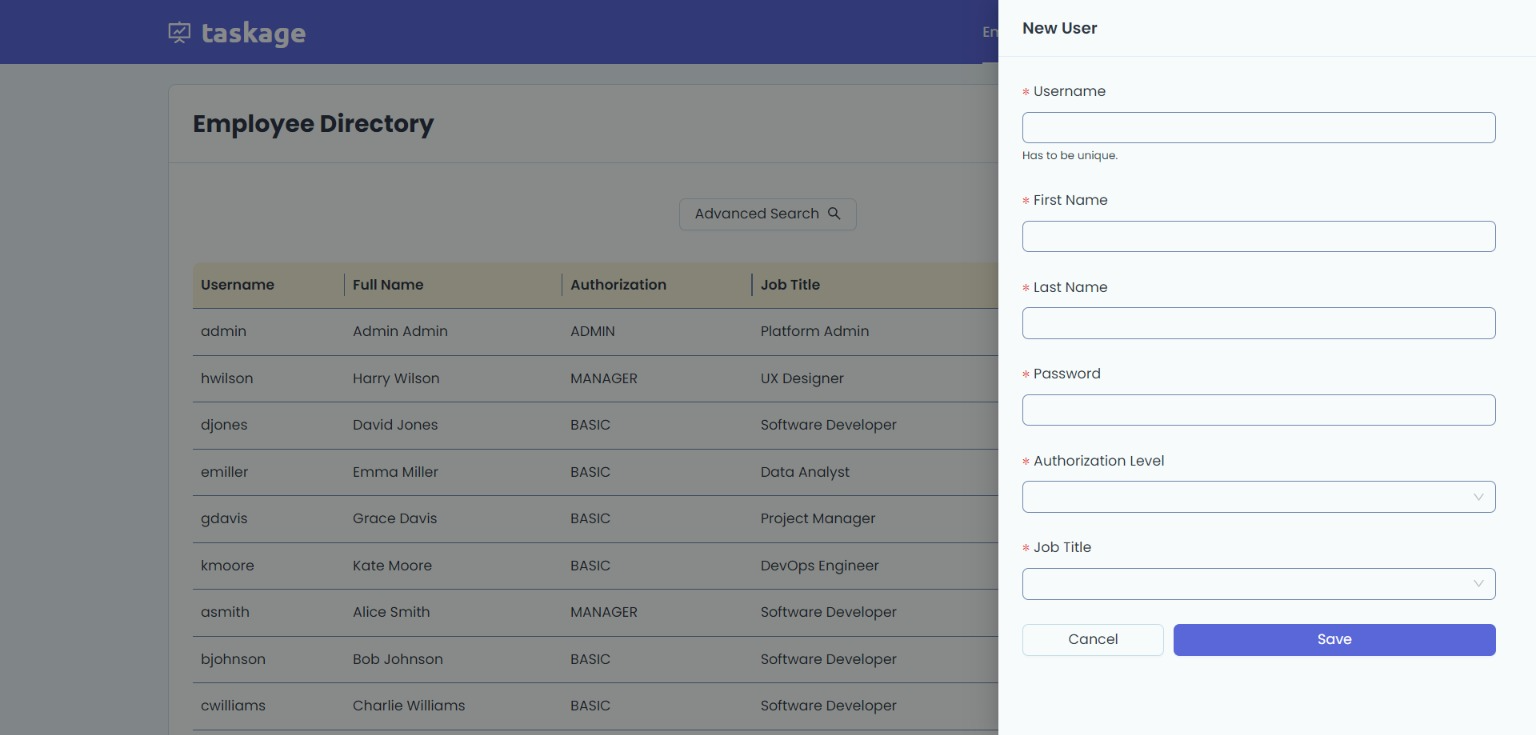
\includegraphics[width=\linewidth]{create-user-form.png}
	\caption{Formularul de creare a unui cont de utilizator}
	\label{fig:user-form-create}
 \end{figure}

Printre opțiunile oferite de caseta de selectare de Job Title se numără și posibilitatea de a salva o nouă titulatură de post, având în vedere că acestea pot varia de la organizație la organizație, în funcție de specific, și nu sunt hard-coded(figura \ref{fig:create-job-title}).

 \begin{figure}[H]
	\centering
 	 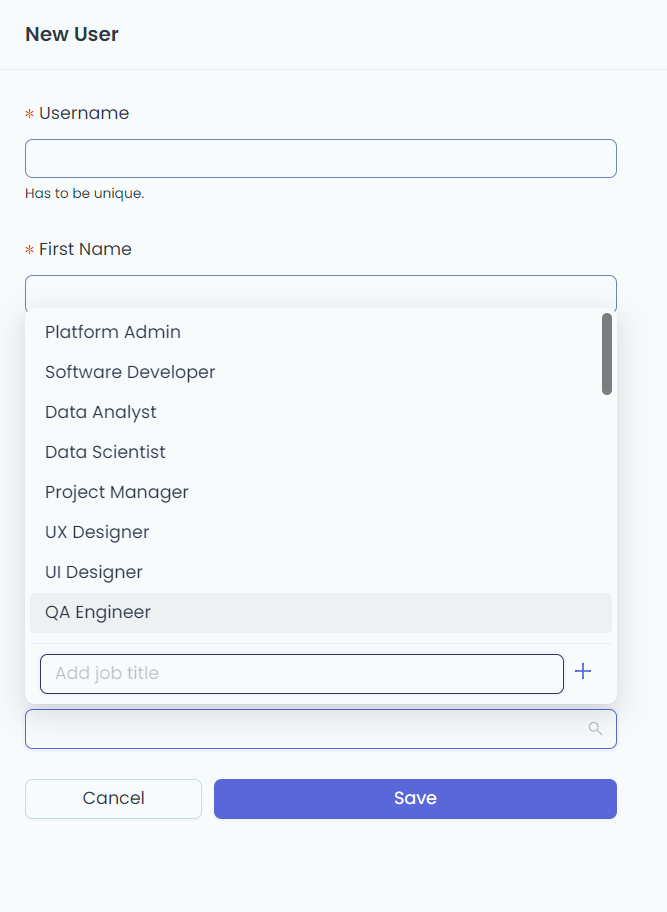
\includegraphics[width=0.5\linewidth]{create-job-title.png}
	\caption{Funcționalitatea de creare a unei noi titulaturi}
	\label{fig:create-job-title}
 \end{figure}

Formularul de actualizare este deschis prin apăsarea pictogramei în formă de creion de pe linia tabelului corespunzătoare contului ce se vrea modificat. Acesta ascunde valoarea câmpului cu parola, dar permite schimbarea ei împreună cu orice detaliu al contului. De asemenea, în colțul din dreapta sus se află butonul ce oferă posibilitatea de ștergere a contului.

 \begin{figure}[H]
	\centering
 	 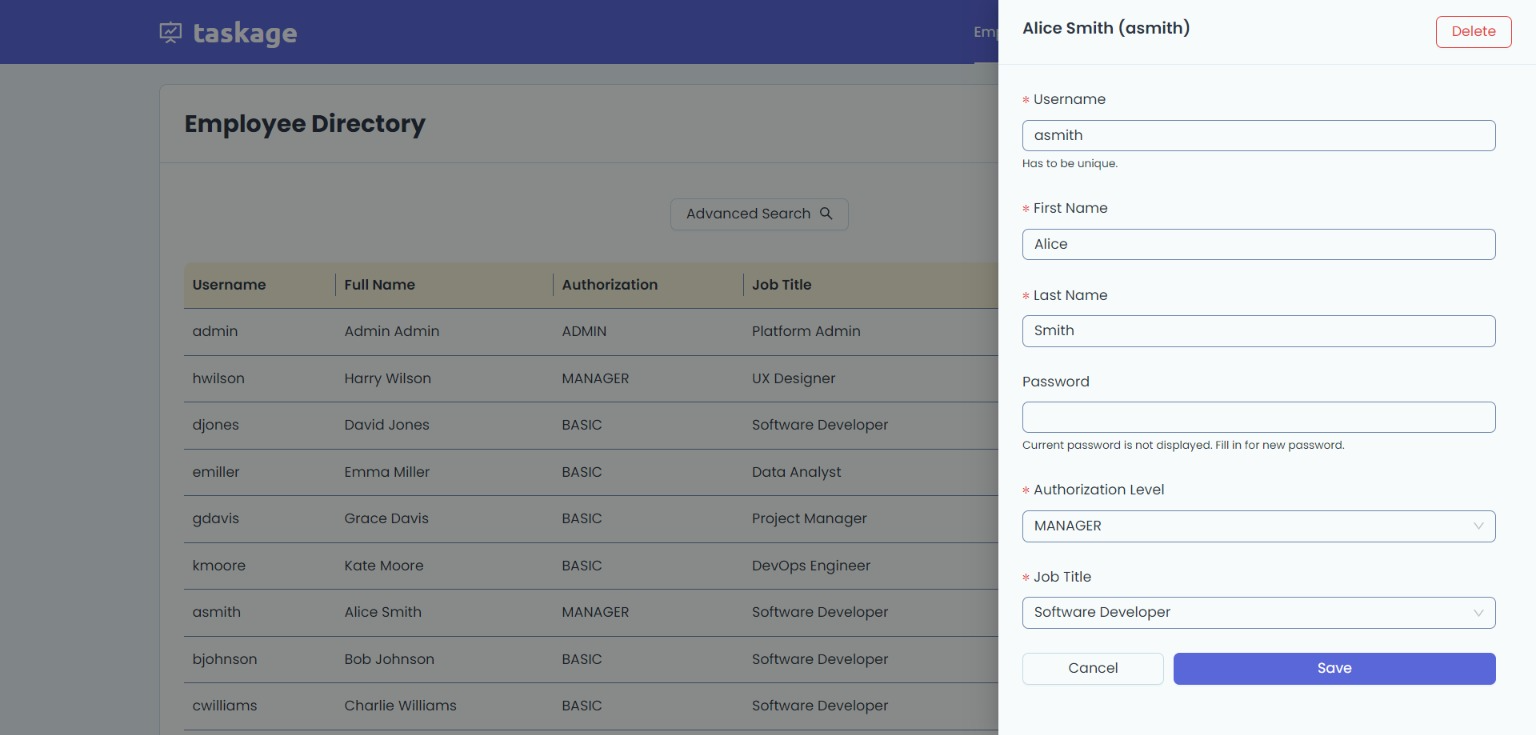
\includegraphics[width=\linewidth]{update-user-form.png}
	\caption{Formularul de actualizare a unui cont de utilizator}
	\label{fig:user-form-update}
 \end{figure}

În mod similar, administratorul are acces la „Team Manager”(figura \ref{fig:team-manager}), unde poate efectua operații similare, dar pentru echipe și componența lor. Echipele sunt prezentate sub forma unui tabel paginat care prezintă datele cele mai semnificative despre fiecare echipă, reprezentative pentru identificare: numele echipei și manager-ul(numit team lead în cadrul interfeței). Pentru vizualizarea celorlalte detalii ale echipei, este necesară apăsarea pictogramei din coloana „View” pentru echipa dorită.

 \begin{figure}[H]
	\centering
 	 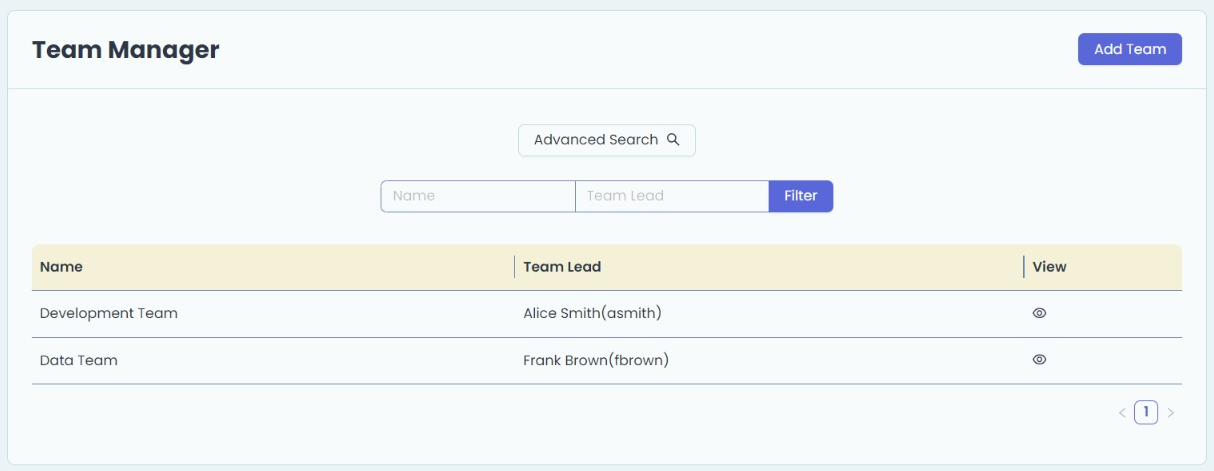
\includegraphics[width=\linewidth]{team-manager-1.png}
	\caption{Team Manager}
	\label{fig:team-manager}
 \end{figure}

Odată cu apăsarea acestei pictograme, se va deschide un side panel cu informațiile complete(figura \ref{fig:team-panel-read}). Acesta este, la fel ca cel de creare a unui cont de utilizator, generic, în sensul în care se randează, atât sub forma de vizualizare, cât și sub alte două moduri: creare și editare(figura \ref{fig:team-panel}). Formularele au restricții specifice. De exemplu, un utilizator poate fi membru al unei singure echipe, iar numele echipei trebuie să fie unic.

 \begin{figure}[H]
	\centering
	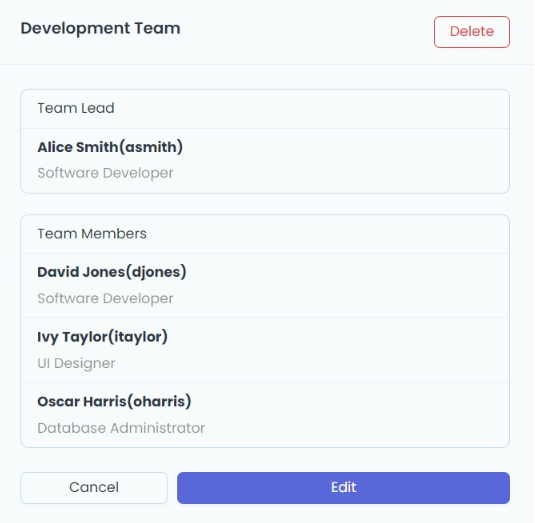
\includegraphics[width=0.5\linewidth]{team-read-1.png}
	\caption{Side panel de echipă sub forma de vizualizare}
	\label{fig:team-panel-read}
 \end{figure}

 \begin{figure}[H]
 	 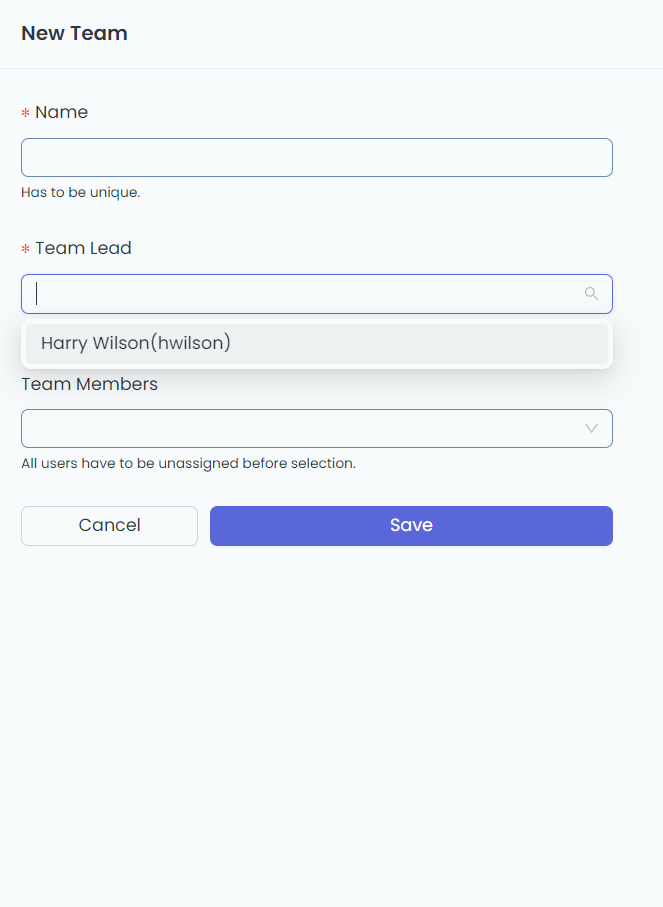
\includegraphics[width=0.5\linewidth]{team-create-1.png}
	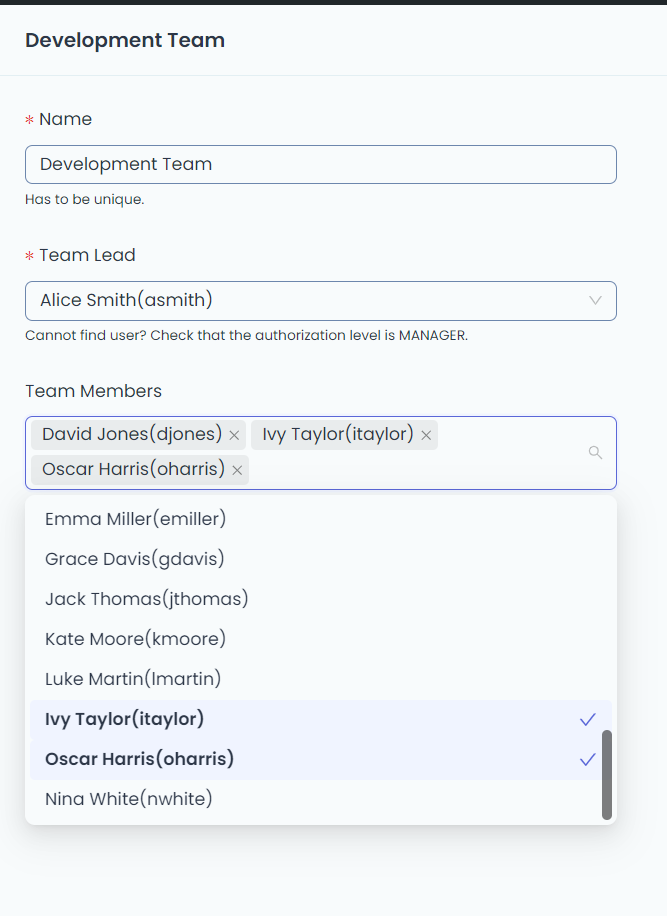
\includegraphics[width=0.5\linewidth]{team-update-1.png}
	\caption{Side panel de echipă sub formele: creare, editare}
	\label{fig:team-panel}
 \end{figure}

De asemenea, administratorul dispune de o pagina numită „My Metrics”(figura \ref{fig:my-metrics}) unde poate vizualiza componenta „Admin Dashboard”.

 \begin{figure}[H]
	\centering
 	 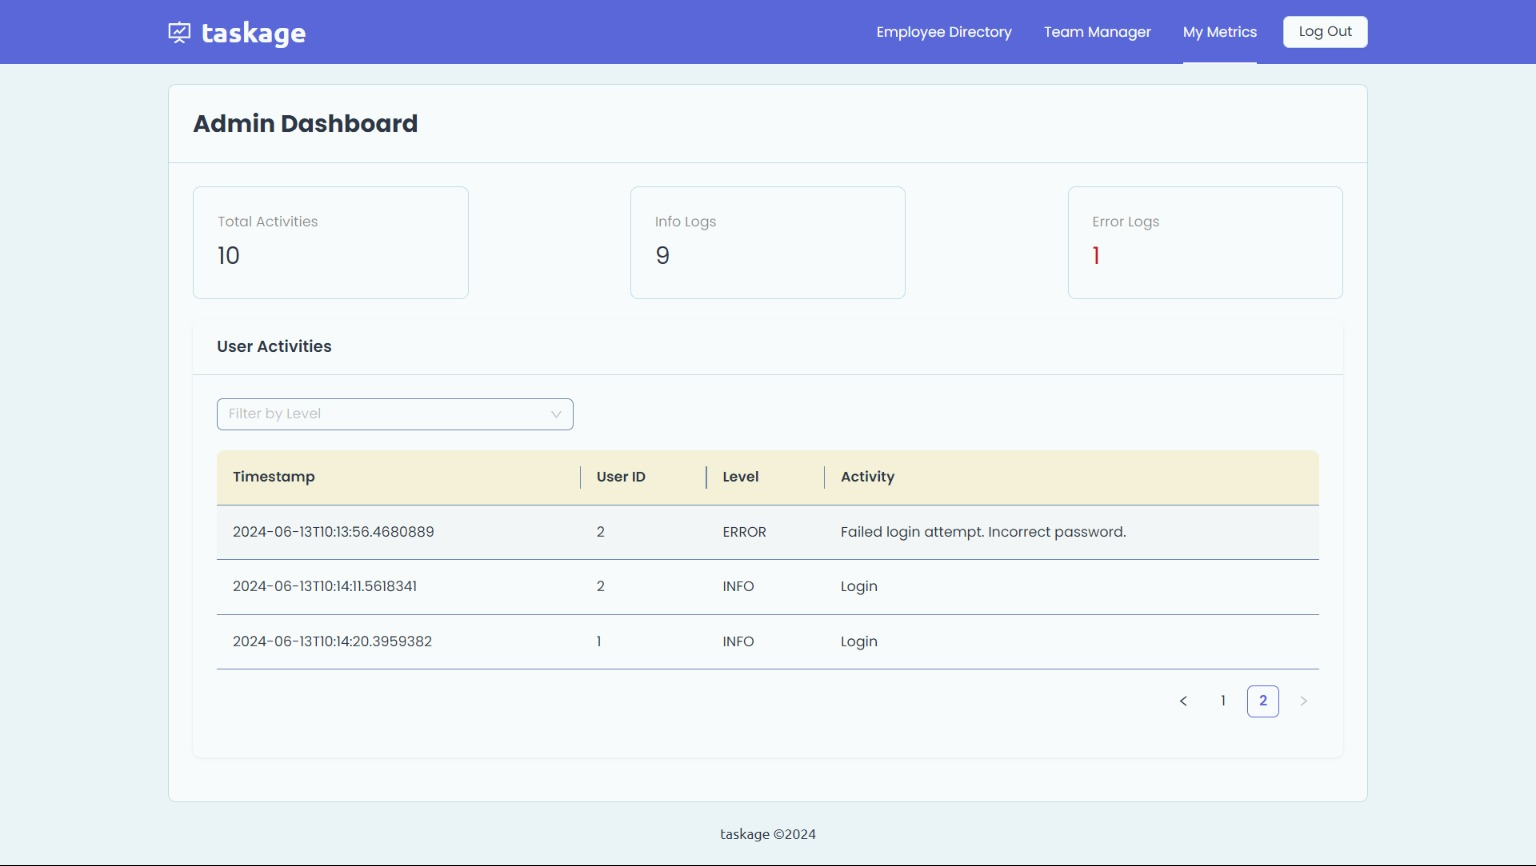
\includegraphics[width=\linewidth]{my-metrics.png}
	\caption{Pagina „My Metrics”}
	\label{fig:my-metrics}
 \end{figure}

De pe această pagină, administratorul află informații despre utilizarea platformei, poate urmări activitatea utilizatorilor și eventualele erori întâmpinate în cadrul unui tabel cu informații despre când, cine și ce activitate a declanșat, primind o imagine de ansamblu asupra gradului de utilizare și eficiență al platformei.

\section{Funcționalitățile rolului de manager}

Utilizatorul cu rol de manager are la dispoziție două componente principale: „Sprint Dashboard” și „Team Details”. După autentificare, este redirecționat către „Sprint Dashboard”, adică panoul de sprint(figura \ref{fig:sprint-dashboard}) al propriei echipe, care funcționează ca un intrument de gestiune a sarcinilor de lucru și a sprinturilor.

Aici, utilizatorul poate vizualiza toate sarcinile de lucru încadrate în sprintul curent, grupate după statusul lor: To Do, In Progress și Done. În cadrul acestei interfețe sunt afișate informațiile esențiale unui task, și anume titlu, prioritate, membru al echipei asignat și progres.

 \begin{figure}[H]
	\centering
 	 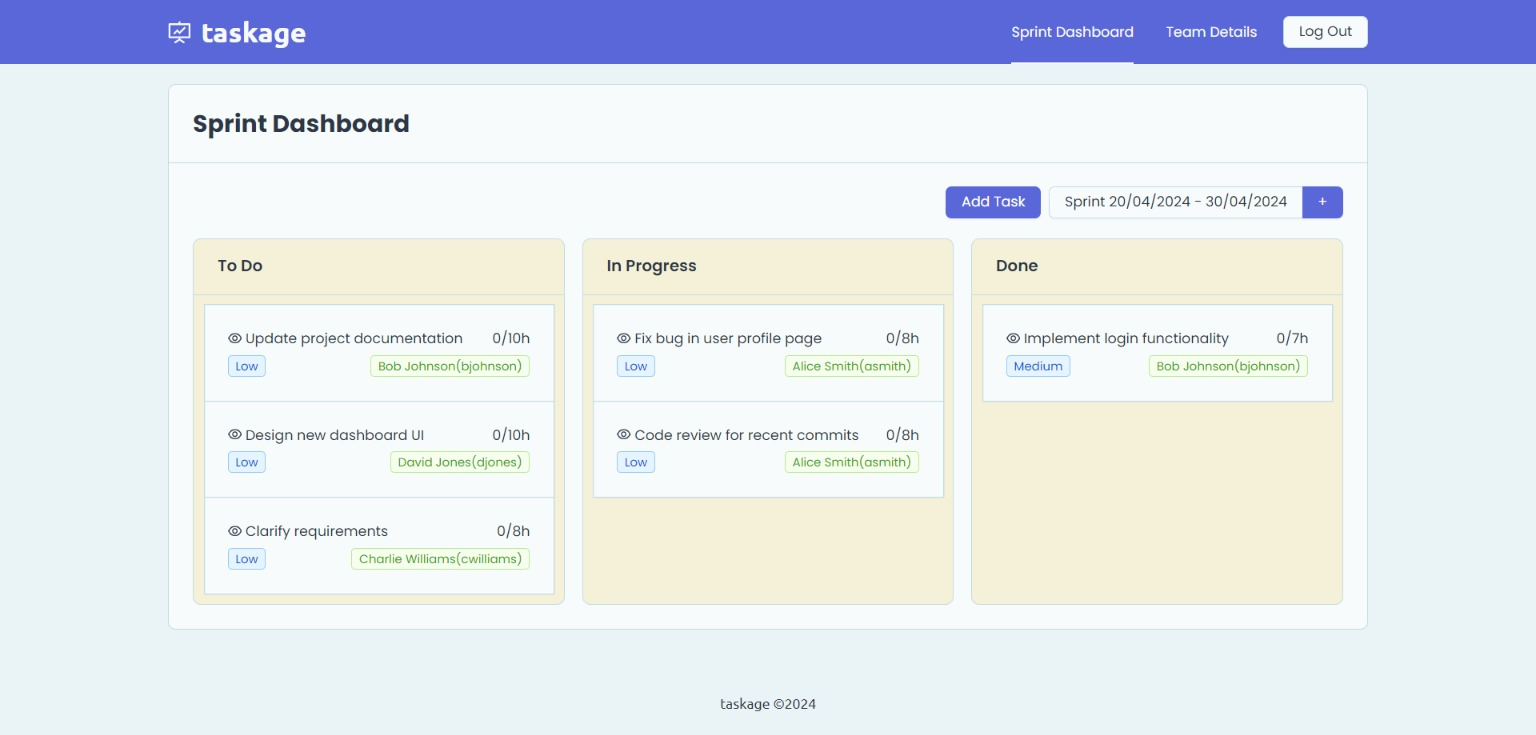
\includegraphics[width=\linewidth]{sprint-dashboard.png}
	\caption{„Sprint Dashboard” - panoul de sprint}
	\label{fig:sprint-dashboard}
 \end{figure}

Pentru vizualizarea celorlalte informații referitoare la task(puncte de efort, tip de task, descriere), manager-ul trebuie să apese pictograma de langă titlul task-ului dorit, care va deschide un side panel ca cel din figura \ref{fig:task-view}, care poate trece în modul de editare prin apăsarea butonului „Edit”.

 \begin{figure}[H]
	\centering
 	 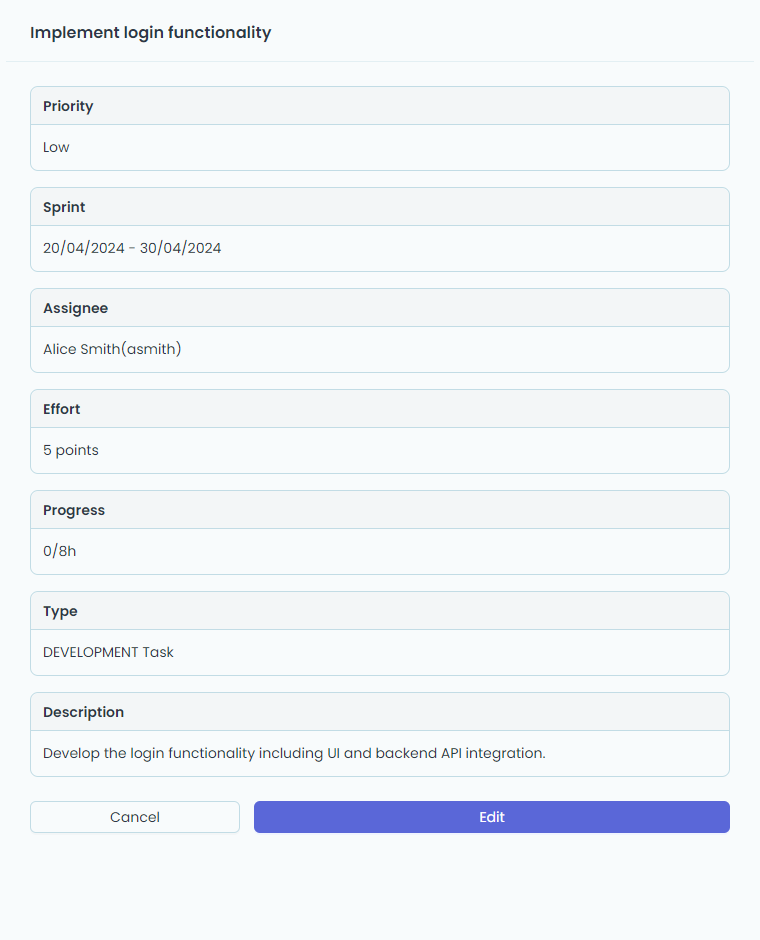
\includegraphics[width=0.5\linewidth]{task-view.png}
	\caption{Side panel cu detaliile sarcinii de lucru}
	\label{fig:task-view}
 \end{figure}

Pentru crearea unui nou task, utilizatorul apasă butonul „Add Task” de pe aceeași pagină, care va deschide într-un side panel formularul din figura \ref{fig:task-create}.

 \begin{figure}[H]
	\centering
 	 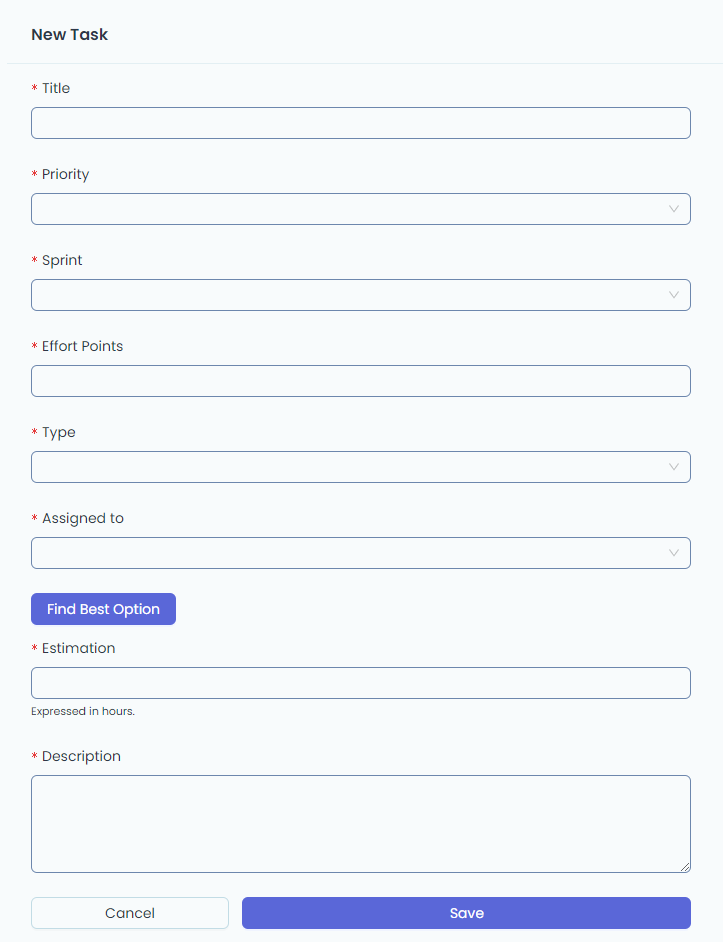
\includegraphics[width=0.5\linewidth]{task-create.png}
	\caption{Formularul de creare a unei sarcini de lucru}
	\label{fig:task-create}
 \end{figure}

Funcționalitatea implementată de Taskage-Helper, descrisă în secțiunea 4.6, este utilizată în cadrul acestui formular. Butonul „Find Best Option” declanșează generarea unei sugestii, însă pentru calculele de similaritate este nevoie de completarea unor câmpuri esențiale: prioritate, sprint, puncte de efort, tip de sarcină de lucru. În cazul în care aceste câmpuri nu sunt completate, butonul va afișa un mesaj care indică că este nevoie de completarea lor(figura \ref{fig:task-create-disabled}).

 \begin{figure}[H]
	\centering
 	 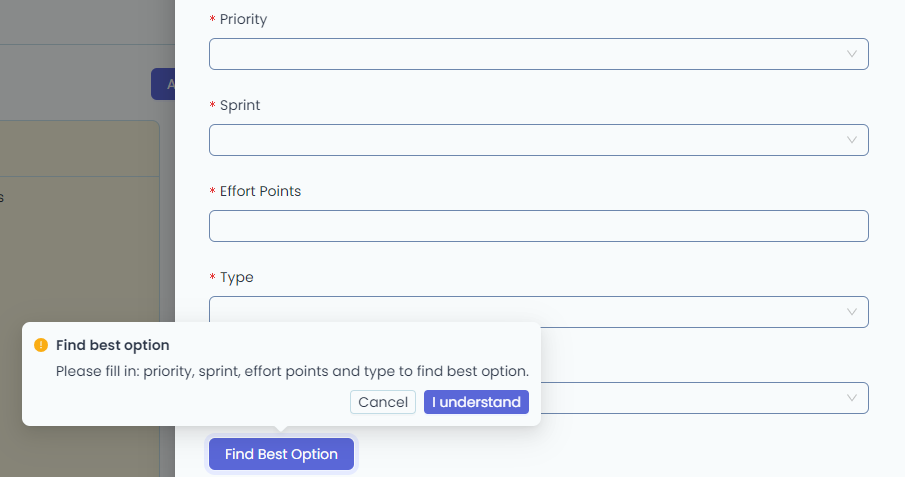
\includegraphics[width=0.7\linewidth]{task-create-disabled.png}
	\caption{Răspunsul „Find Best Option” atunci când nu sunt completate câmpurile necesare}
	\label{fig:task-create-disabled}
 \end{figure}

Dacă aceste câmpuri sunt completate, algoritmul va genera sugestia și o va prezenta cu opțiunile de acceptare, care va selecta automat sugestia pentru câmpul „Assigned to”, sau respingere, pentru eventuală selecție manuală(figura \ref{fig:task-create-enabled}).

 \begin{figure}[H]
	\centering
 	 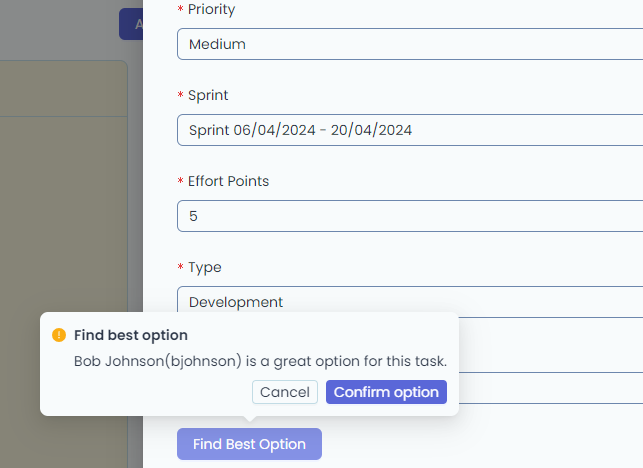
\includegraphics[width=0.7\linewidth]{task-create-enabled.png}
	\caption{Răspunsul „Find Best Option” atunci când sunt completate câmpurile necesare}
	\label{fig:task-create-enabled}
 \end{figure}

De asemenea, utilizatorul poate gestiona sprinturile cu ajutorul setului de componente din figura \ref{fig:new-sprint}. Cu ajutorul primei componente, acesta poate selecta sprint-ul pe care dorește să în vizualizeze cu ajutorul unui meniu drop-down sau poate crea un sprint nou apăsând pe butonul „+”, ce deschide a doua componentă ilustrată, un modal. Mai departe, trebuie să selecteze data de început și data de final a sprintului. Datele pe care le are la dispoziție pentru crearea sprintului sunt datele care urmează ultimului sprint creat, fără să existe posibilitatea de a adăuga sprinturi în trecut, așa cum se poate observa în a treia captură de ecran a figurii, unde parte din calendar este dezactivată.

 \begin{figure}[H]
	\centering
	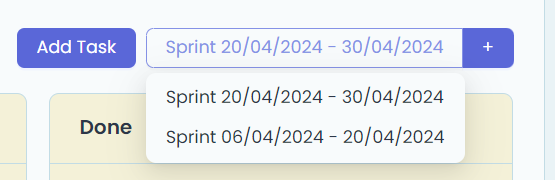
\includegraphics[width=0.5\linewidth]{sprint-dropdown.png}
 	 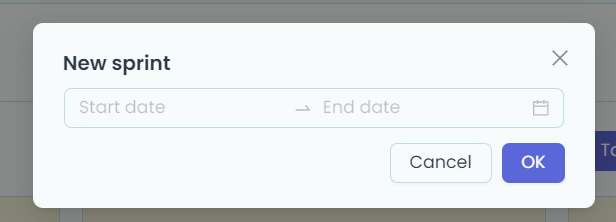
\includegraphics[width=0.5\linewidth]{new-sprint-form.png}
	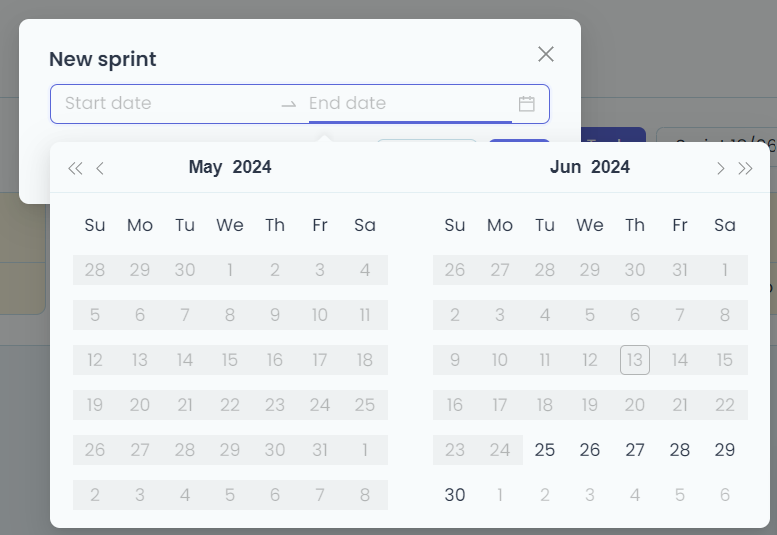
\includegraphics[width=0.5\linewidth]{new-sprint-calendar.png}
	\caption{Componentele pentru gestionarea sprinturilor}
	\label{fig:new-sprint}
 \end{figure}

Tot ce ține de panoul cu sarcini de lucru este actualizat în timp real cu ajutorul WebSockets, mecanism prezentat în secțiunea 4.5. În zona „Network” a Developer Tools din browser, putem vizualiza datele primite prin WebSocket. De exemplu, pentru acțiunea „UPDATE”(figura \ref{fig:task-ws}), sarcina de lucru actualizată se va schimba în timp real pentru toți utilizatorii prezenți pe pagina panoului de task-uri.

 \begin{figure}[H]
	\centering
 	 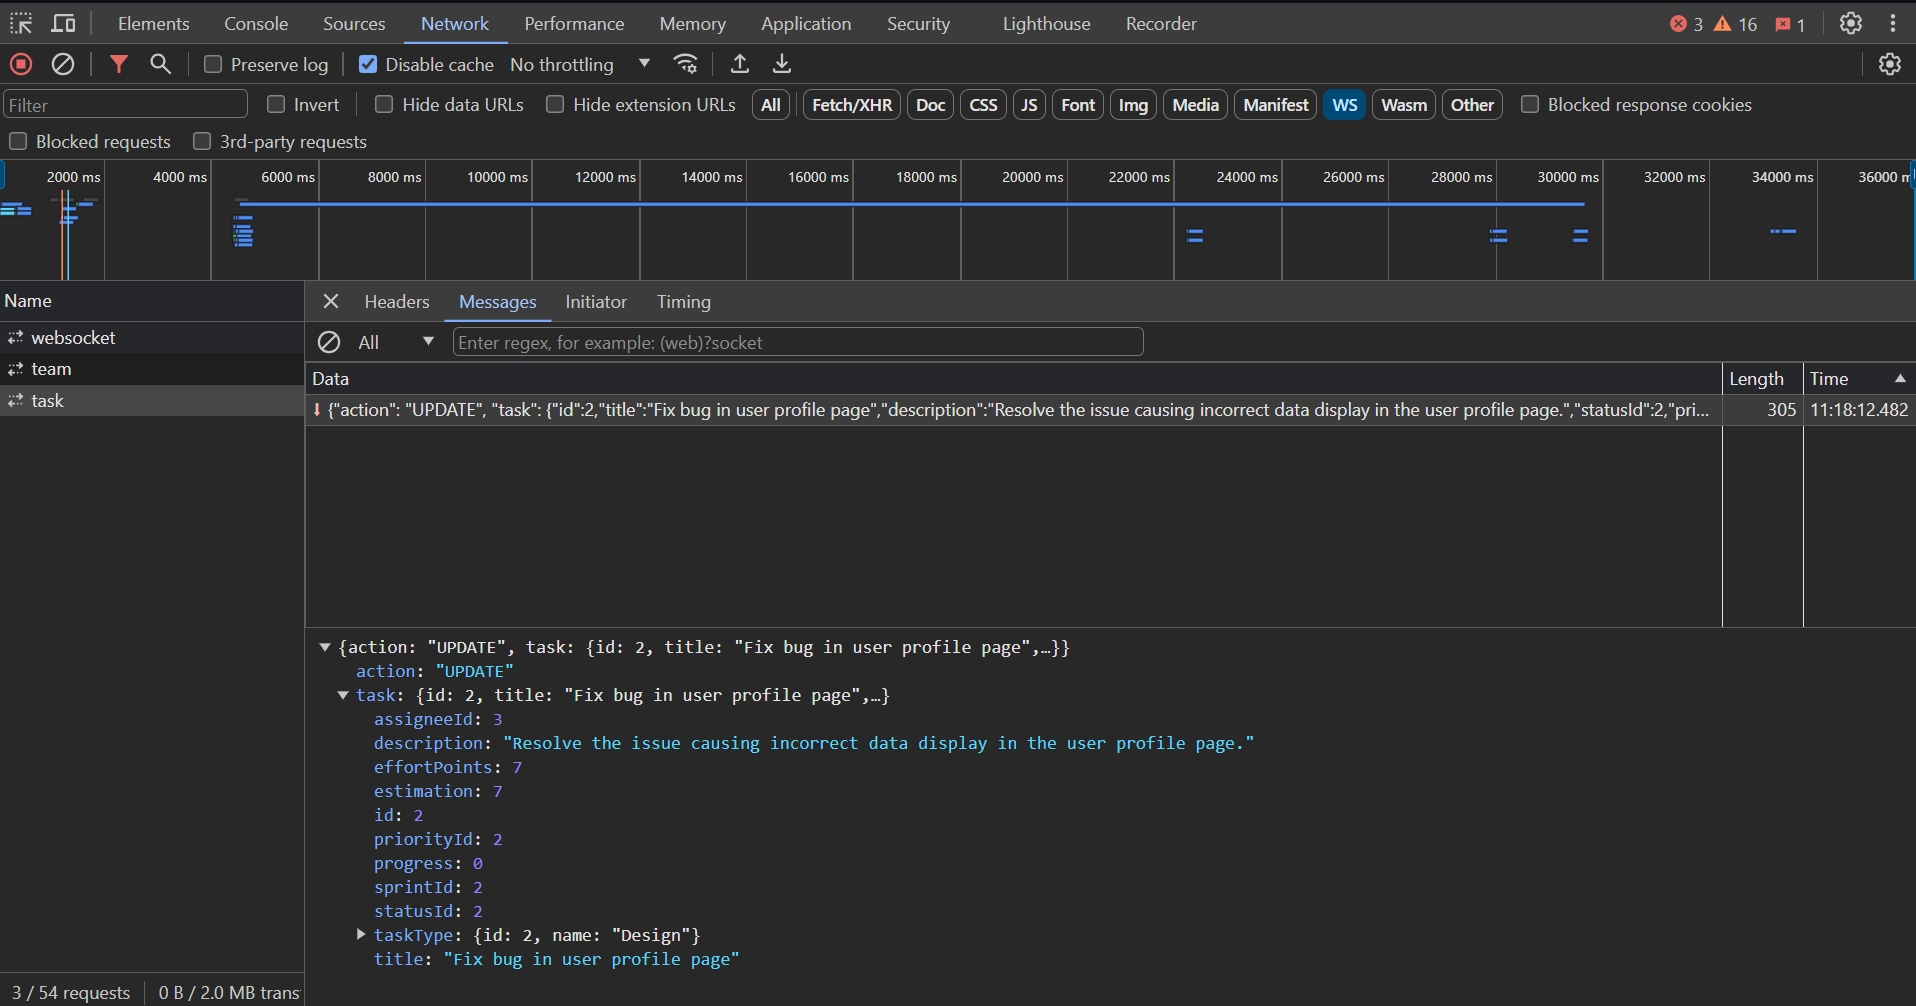
\includegraphics[width=\linewidth]{task-ws.png}
	\caption{Acțiunea „UPDATE” primită prin WebSocket}
	\label{fig:task-ws}
 \end{figure}

Rezultatul acestui mesaj primit prin WebSocket reiese din faptul că, mai mulți utilizatori, sau chiar și mai multe instanțe de browser ale aceluiași utilizator vor fi mereu sincronizate din punct de vedere al datelor afișate(figurile \ref{fig:ws-sync-1} și \ref{fig:ws-sync-2}).

 \begin{figure}[H]
	\centering
 	 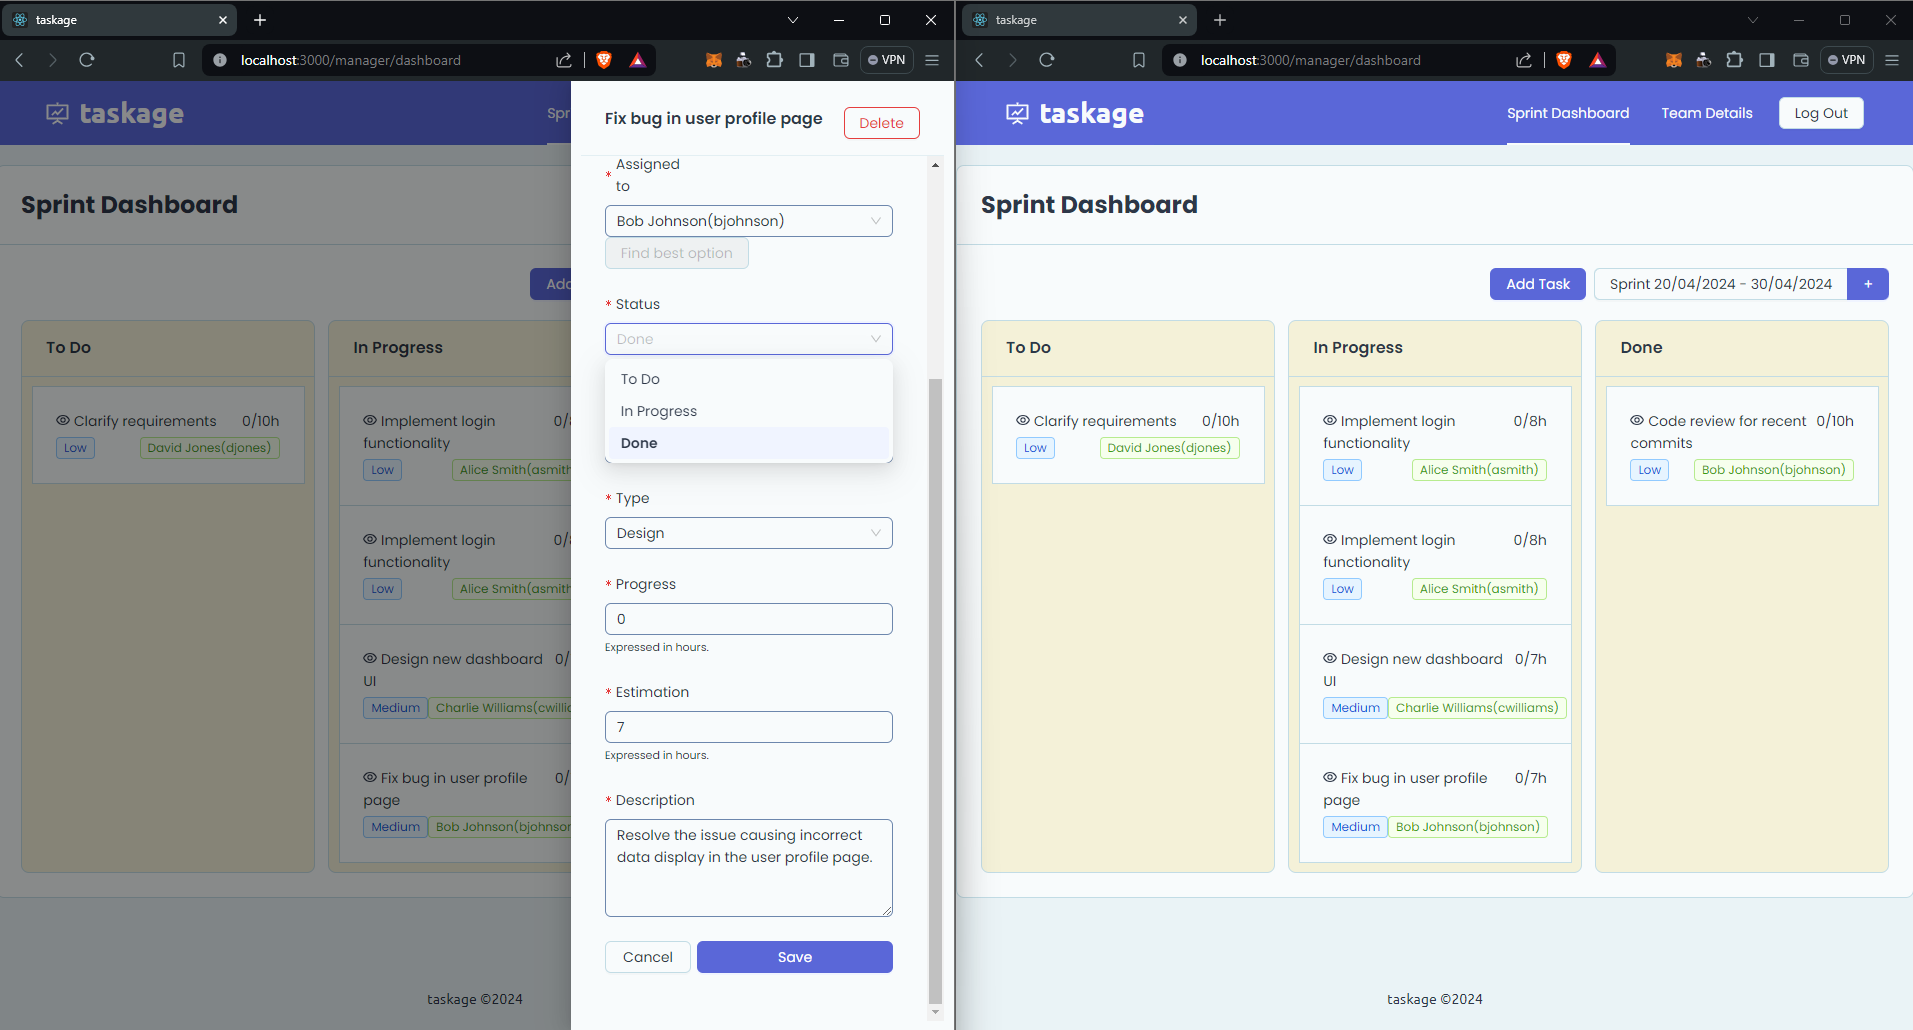
\includegraphics[width=\linewidth]{before-save.png}
	\caption{Acțiunea de actualizare sincronizată}
	\label{fig:ws-sync-1}
 \end{figure}

 \begin{figure}[H]
	\centering
	 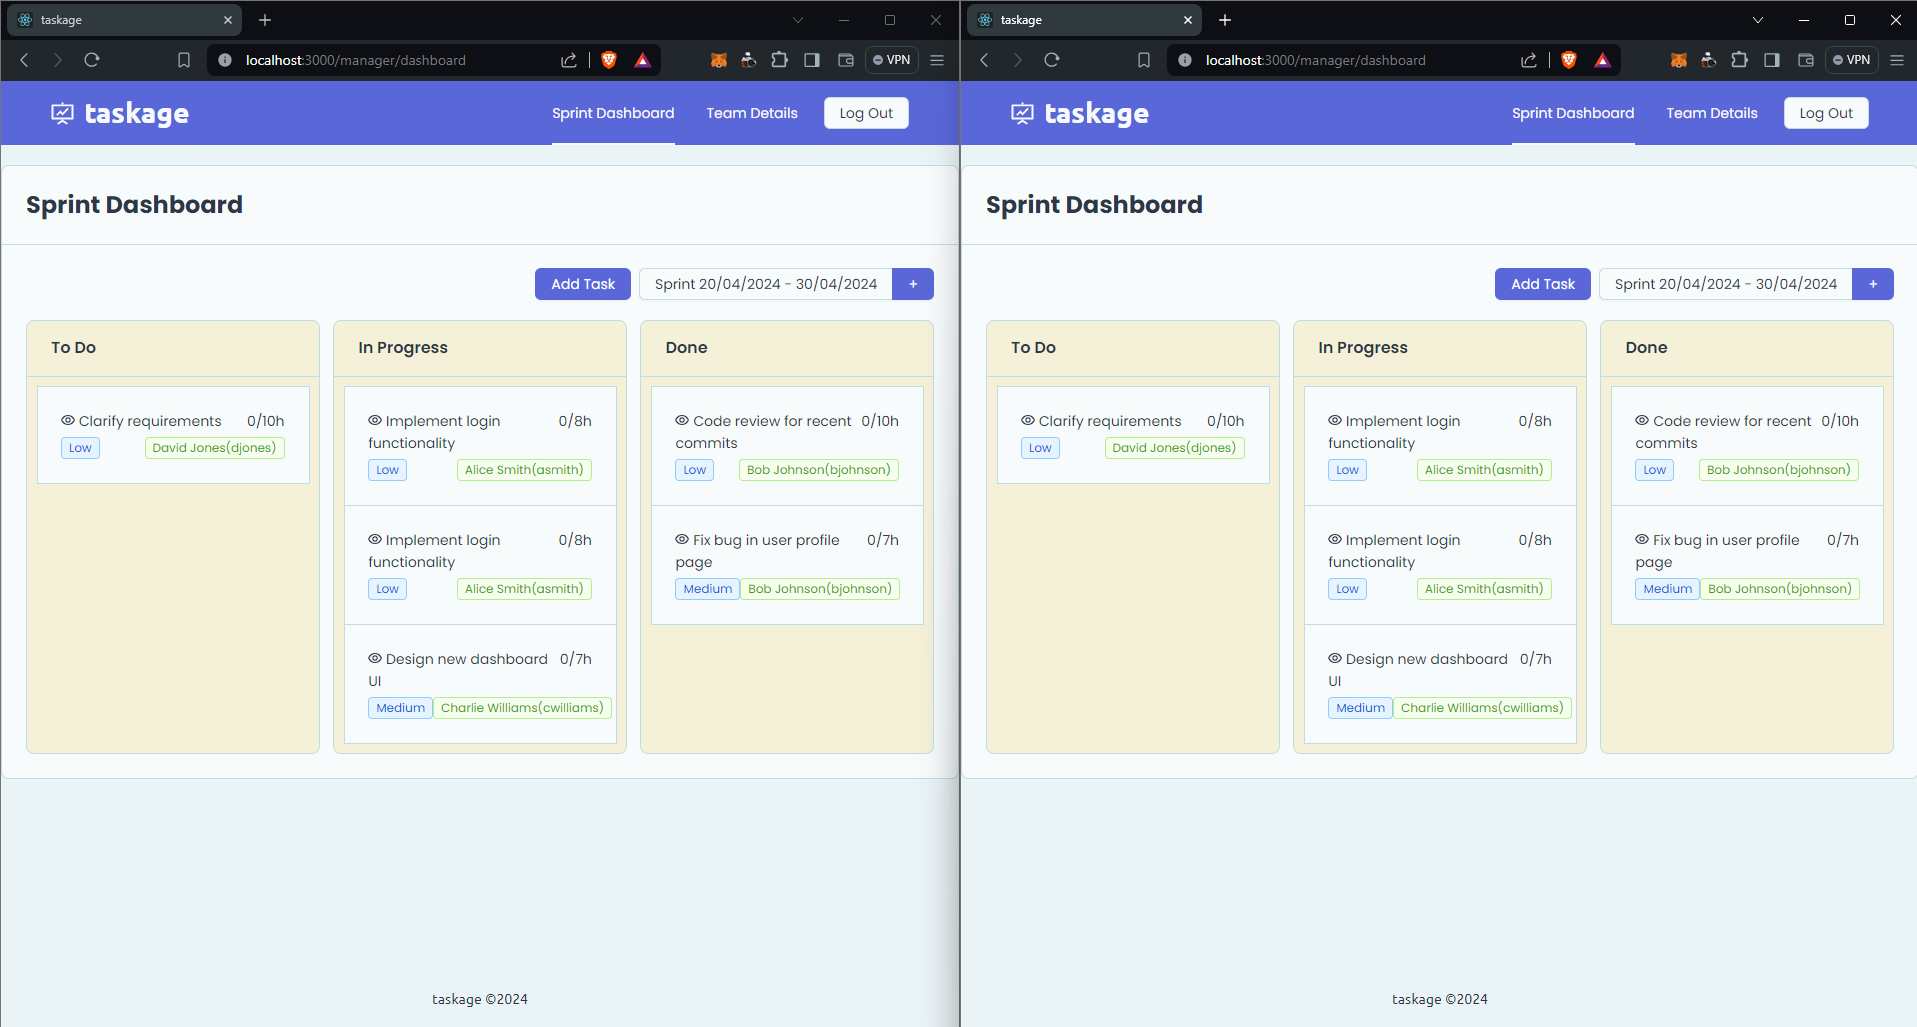
\includegraphics[width=\linewidth]{after-save.png}
	\caption{Rezultatul acțiunii de actualizare sincronizată}
	\label{fig:ws-sync-2}
 \end{figure}

Cealaltă rută, „Team Details”, oferă detalii legat de capacitatea membrilor echipei, calculând raportul dintre numărul total de ore al sprintului și estimările sarcinilor asignate fiecărui membru al echipei(figura \ref{fig:team-details}). Aceste statistici sunt exprimate per sprint, care poate fi selectat dintr-un drop-down reutilizat din componenta „Sprint Dashboard”. Rolul lor este de a facilita alegerea în cazul asignării manuale, reprezând într-un mod de înțeles disponibilitatea fiecărui membru al echipei.

 \begin{figure}[H]
	\centering
 	 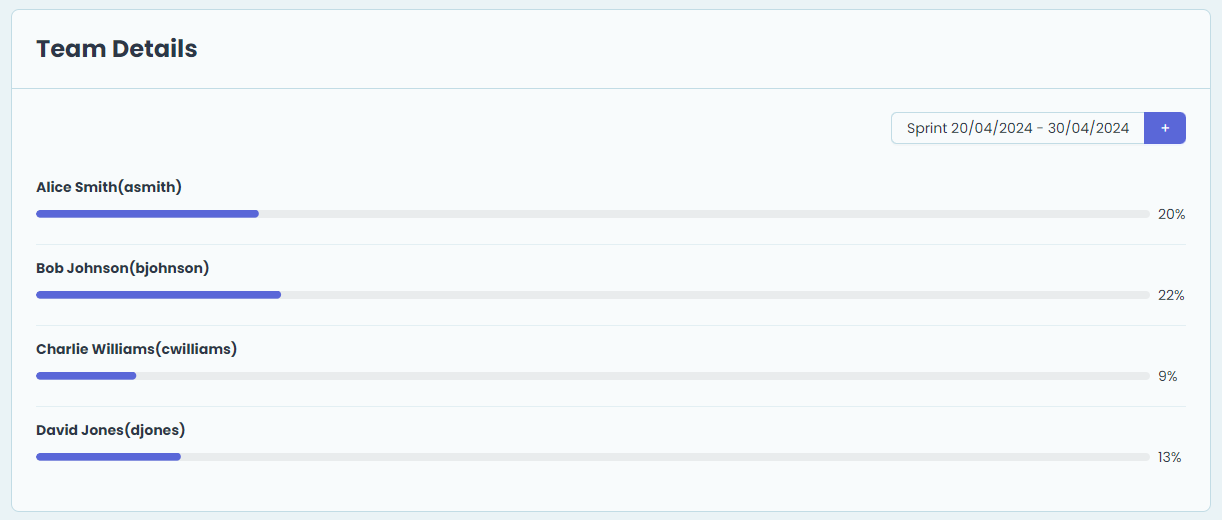
\includegraphics[width=\linewidth]{team-details.png}
	\caption{Statisticile capacității membrilor echipei}
	\label{fig:team-details}
 \end{figure}

\section{Funcționalitățile rolului de membru de echipă}

Utilizatorii simpli dispun de funcționalități asemănătoare managerilor, așa că urmează să expun doar capabilitățile diferite.

Asemănător rolului de manager, după autentificare, utilizatorul simplu este redirecționat către Sprint Dashboard, însă aici își poate vizualiza numai atribuțiile personale(figura \ref{fig:basic-sprint-dashboard}).

 \begin{figure}[H]
	\centering
 	 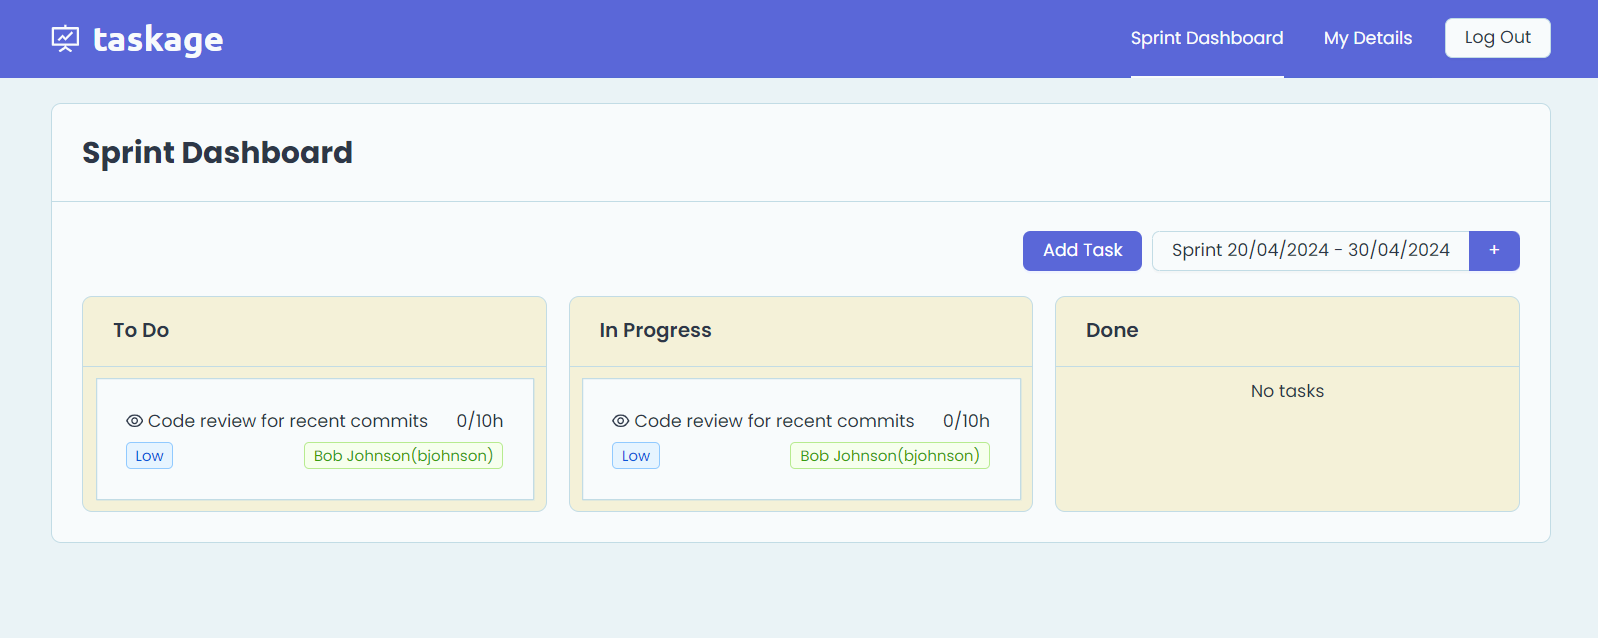
\includegraphics[width=\linewidth]{basic-sprint-dashboard.png}
	\caption{„Sprint Dashboard” din perspectiva unui simplu membru de echipă}
	\label{fig:basic-sprint-dashboard}
 \end{figure}

Acesta primește un nou tip de notificări, prin care este informat atunci când managerul său i-a asignat un nou task(figura \ref{fig:new-task-toast}), ca răspuns la mesajul specific primit prin sistemul WebSocket descris anterior, în secțiunea 4.5.

 \begin{figure}[H]
	\centering
 	 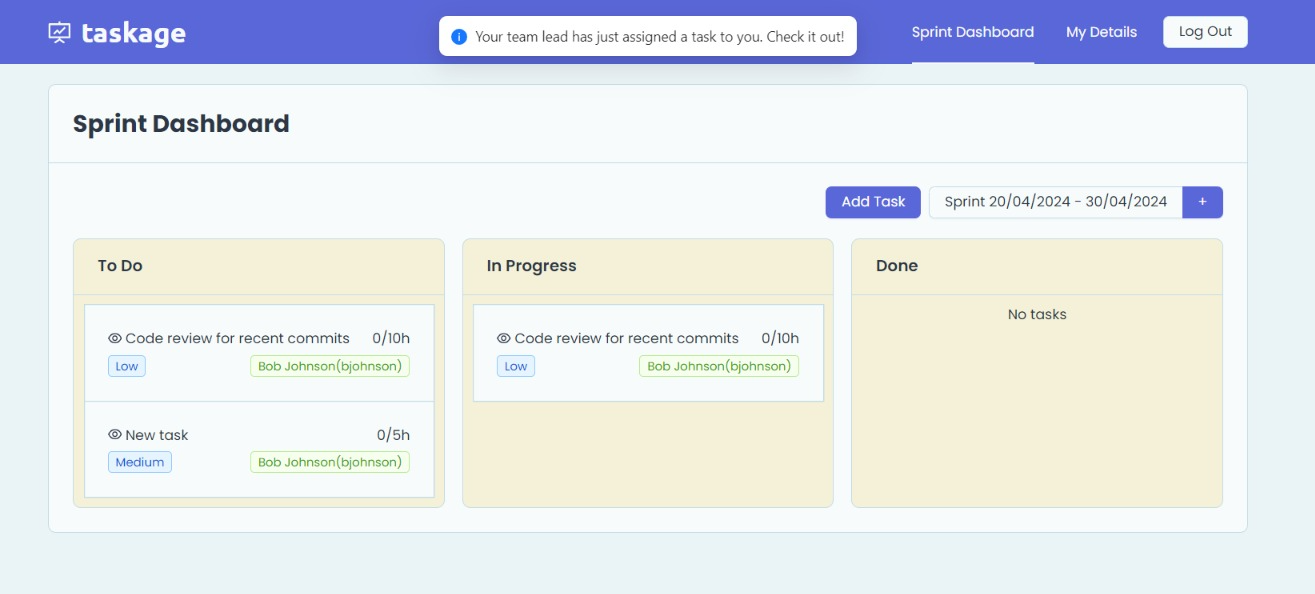
\includegraphics[width=\linewidth]{new-task-toast.png}
	\caption{„New task” în Sprint Dashboard și notificarea aferentă}
	\label{fig:new-task-toast}
 \end{figure}

O altă diferență este vizibilă pe pagina „My details”, care este o variantă personalizată a „Team Details”. Aici, utilizatorul poate să vadă, măsurată, performanța sa pe parcursul ultimelor cinci sprinturi și capacitatea sprintului curent, raportată la sarcinile de lucru care i-au fost asignate și estimările lor(figura \ref{fig:my-stats}).

 \begin{figure}[H]
	\centering
 	 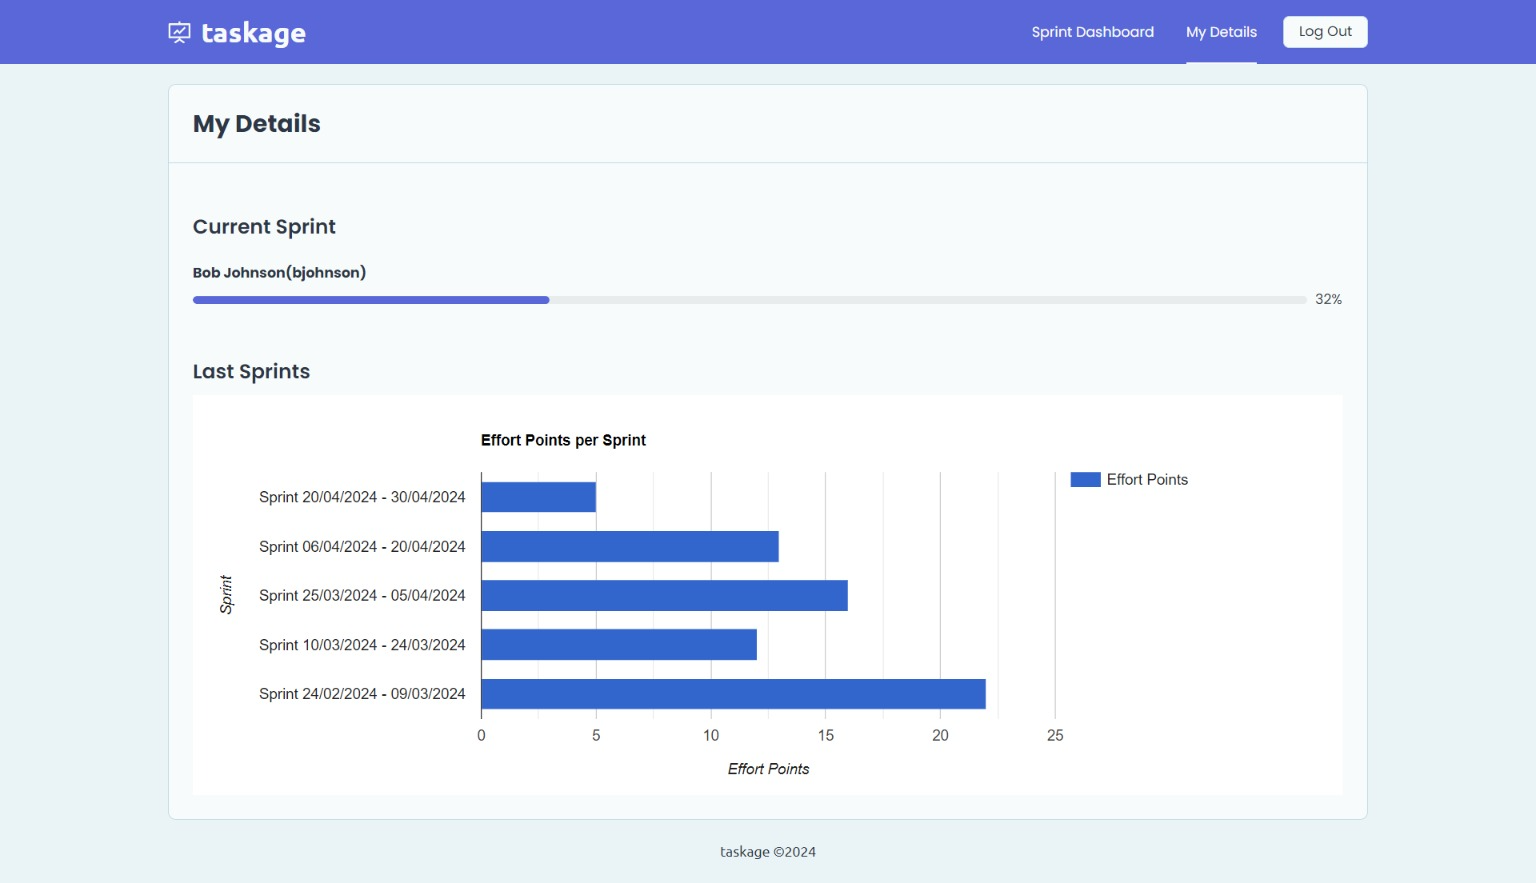
\includegraphics[width=\linewidth]{my-stats.png}
	\caption{Pagina de statistici a unui utilizator simplu}
	\label{fig:my-stats}
 \end{figure}

\chapter{Concluzii}

În concluzie, aplicația Taskage reușeste ceea ce își propune, și anume să reprezinte o alternativă viabilă la toate celelalte aplicații ce permit utilizatorilor doar să-și creeze sarcini de lucru și să le asigneze, automatizând procesul din urmă, pe baza performanțelor trecute ale utilizatorilor, venind cu o soluție de a distribui volumul de muncă într-un mod eficient, fapt ce ușurează munca unui Scrum Master.

În ceea ce privește posibilele direcții de extindere ale acestei aplicații, îmbunătățirile principale ce pot fi facute gravitează în jurul algoritmului de asignare automată pe sarcina de lucru a invidizilor. Principalul gol ce se evidențiază în algoritmul curent este acela că nu ia în considerare frecvența fiecărui tip de însărcinare pentru membrii echipei, astfel neluând în considerare intrări aparent duplicate, cu caracteristici similare. 

În scopul rezolvării acestui punct slab din algoritm putem introduce o nouă metrică ce ia in considerare frecvența de apariție a fiecărui tip de sarcină. O modalitate de a implementa această nouă metrică poate viza calculul proporției tipurilor de task pentru fiecare utilizator în parte, astfel integrând în calculul similarității o modalitate de a inclina sistemul să asigneze o sarcină unui membru al echipei cu mai multă experiență cu tipul respectiv de sarcină.

O altă direcție pentru extinderea aplicației poate fi reprezentată de un mod de a preveni utilizatorii de a intra în burnout, asigurându-se că un membru al echipei nu primește mereu același fel de sarcină, cum ar fi rezolvarea unor defecte. Îmbunătățiri ce ar putea fi aduse aplicației implică atât un mod de a asigna tipuri suficient de variate de sarcini utilizatorilor, cât și adăugarea unui tip de monitorizare al productivității membrilor din echipe, pentru a putea observa și preveni intrarea unuia dintre angajați într-o stare de burnout, judecând după volumul de sarcini completate într-o anumită perioadă de timp.

În final, se poate trage concluzia că o aplicație de gestionare eficientă a sarcinilor de lucru poate fi benefică, în special în contexte în care este aplicată metodologia Agile, pentru a asigura un maxim de performanță și eficiență al angajaților, în scopul maximizării atât al productivității, cât și al fericirii angajaților.

\printbibliography[heading=bibintoc]

\end{document}